\documentclass[%
candidate, % тип документа
subf, % подключить и настроить пакет subfig для вложенной нумерации рисунков
%href, % подключить и настроить пакет hyperref
%colorlinks=true % цветные гиперссылки
times % шрифт Times как основной
%,fixint=false % отключить прямые знаки интегралов
]{disser}
\setlength{\parindent}{1.25cm}
\usepackage[a4paper,left=3cm, right=1cm, top=2cm, bottom=2cm, headsep=0.7cm, footskip=1cm]{geometry} %добавить 14pt

\usepackage[T2A]{fontenc}
\usepackage{indentfirst}
\usepackage[utf8]{inputenc}
\usepackage[english,russian]{babel}
\renewcommand{\rmdefault}{ftm}
\usepackage{pdfpages}
\ifpdf\usepackage{epstopdf}\fi
%\renewcommand{\thesectionfont}{\normalsize}
\renewcommand{\sectionfont}{\normalsize}
%\usepackage{caption} % подписи к рисункам в русской типографской традиции
\usepackage{dcolumn}
\linespread{1.6}
%\usepackage{floatrow}
\usepackage{bm}
%\floatsetup[table]{capposition=top}
\usepackage{cmap}
%\usepackage{hyperref}
\usepackage{color}
\usepackage{epstopdf}
\usepackage{floatrow}
\usepackage{amsmath}
\usepackage{lipsum}
\usepackage{amssymb}
\newlength\mysep
\setlength\mysep{0em}% default equivalent to capbesidesep=none
\DeclareFloatSeparators{mysep}%
{\hskip\mysep}
\usepackage{cite}
\usepackage[margin=10pt,font=small,labelsep=endash, figurename= {Рисунок}]{caption}
\usepackage{multirow}
\usepackage{titlesec}
\usepackage{tocloft}
\renewcommand{\cfttoctitlefont}{\hspace{0.38\textwidth} \bfseries\MakeUppercase}
\renewcommand{\cftbeforetoctitleskip}{-1em}
\renewcommand{\cftaftertoctitleskip}{25mm}
\renewcommand{\cftaftertoctitle}{\mbox{}\hfill \\ \mbox{}\hfill{\normalsize с.}\vspace{-4em}}
\cftsetpnumwidth{5mm}
\renewcommand{\cftchappagefont}{\normalfont}
\renewcommand{\cftchapfont}{\normalsize \MakeUppercase{\chaptername} }
\renewcommand\cftchapdotsep{\cftdot} %добавляет отточия после \chapter{title}
\renewcommand{\cftchapleader}{\cftdotfill{\cftchapdotsep}} %делает отточия после \chapter{title} тонкими, (по умолчанию жирные).
\setlength{\cftchapindent}{1mm} %отступ между левым полем и \chapter{}
\setlength{\cftsecindent}{1.25cm} %отступ между левым полем и \section{title}
\setlength{\cftsubsecindent}{2.5cm}
%\renewcommand{\cftsecfont}{\hspace{0pt}}
%\renewcommand{\cftsubsecfont}{\hspace{0pt}}
%\renewcommand{\cftbeforechapskip}{2pt}
%\renewcommand{\cftparskip}{-1mm}
\setlength{\cftbeforechapskip}{1.5pt} %отступ между главами
\setlength{\cftbeforesecskip}{1.5pt} %отступ между секциями \section{title}
\renewcommand{\cftdotsep}{0.5}
\addto\captionsrussian{\renewcommand{\chaptername}{}}
\usepackage{lscape}
\usepackage[font={normal}]{caption}
\renewcommand{\baselinestretch}{1.7}
\usepackage{setspace}
%\onehalfspacing
\usepackage{fancyhdr}
%\usepackage{tempora}
\usepackage[square,numbers,sort&compress]{natbib}
%\usepackage{pscyr}
\usepackage{enumitem}
\setlist{nolistsep, itemsep=0.3cm,parsep=0pt}
\pagestyle{fancy}
\fancyhf{}
\cfoot{\thepage}
\renewcommand{\headrulewidth}{0pt}
\fancypagestyle{plain}{
	\fancyhf{}
	\cfoot{\thepage}
	\renewcommand{\headrulewidth}{0pt}}
\setcounter{page}{5} % начать нумерацию страниц с №2
\usepackage[onehalfspacing]{setspace}
%\captionsetup{format=hang,labelsep=period}
% Использовать полужирное начертание для векторов
% Включать подсекции в оглавление
\setcounter{tocdepth}{3}
%\setcounter{secnumdepth}{2}
\graphicspath{{fig/}}
\titleformat{\section}[block]{\bfseries\normalsize}{\hspace{1.25cm}\thesection}{1ex}{}
\titlespacing{\section}{0mm}{8.466mm}{12.7mm}
\titleformat{\subsection}{\normalfont\fontsize{15}{14}}{\thesubsection}{1ex}{}
\titlespacing{\subsection}{1.25cm}{8.466mm}{12.7mm}
\titleformat{\subsubsection}{\normalfont\fontsize{15}{14}}{\thesubsubsection}{1ex}{}
\titlespacing{\subsubsection}{\parindent}{8.466mm}{8.466mm}
%\floatsetup[table]{capposition=beside,capbesideposition={left}}
\makeatletter
\renewenvironment{thebibliography}[1]
{\centering {СПИСОК ИСПОЛЬЗОВАННЫХ ИСТОЧНИКОВ}
	\@mkboth{\MakeUppercase\refname}{\MakeUppercase\refname}%
	\list{\@biblabel{\@arabic\c@enumiv}}%
	{\settowidth\labelwidth{\@biblabel{#1}}%
		\setlength{\itemindent}{\dimexpr\labelwidth+\labelsep+1.25cm}
		\leftmargin\z@
		\@openbib@code
		\usecounter{enumiv}%
		\let\p@enumiv\@empty
		\renewcommand\theenumiv{\@arabic\c@enumiv}}%
	\sloppy
	\clubpenalty4000
	\@clubpenalty \clubpenalty
	\widowpenalty4000%
	\sfcode`\.\@m}
{\def\@noitemerr
	{\@latex@warning{Empty `thebibliography' environment}}%
	\endlist}
\makeatother
\captionsetup[table]{singlelinecheck=false,justification=raggedright}
\floatsetup[table]{capposition=top}
\linespread{1.4}
\begin{document}
	%\newpage
\begin{center}
РЕФЕРАТ
\end{center}
\vspace{6mm}
%\refstepcounter{chapter}
%\addcontentsline{toc}{chapter}{РЕФЕРАТ}

Расчетно-пояснительная записка 78 с., 24 рис., 4 табл., 30 источн. 

СЛУХОВОЕ ВОСПРИЯТИЕ, ГЕМОДИНАМИЧЕСКИЕ ПАРАМЕТРЫ, ОПТИЧЕСКИЕ СВОЙСТВА БИОЛОГИЧЕСКИХ ТКАНЕЙ, РАЗРАБОТКА КОНСТРУКЦИИ БЛОКА БТС, МЕТОД СПЕКТРОФОТОМЕТРИИ, ФУНКЦИОНАЛЬНАЯ АКТИВНОСТЬ ГОЛОВНОГО МОЗГА.

Работа включает в себя медико-биологическую, проектно-конструкторскую и исследовательскую части.

Объектом разработки является биотехническая система объективного контроля слухового восприятия спектрофотометрическим методом.

Предмет – блок БТС, обеспечивающий одновременную подачу звукового сигнала и работу спектрофотометрических датчиков в непрерывном режиме.

Цель работы – разработка оптимального конструкторского и схемотехнического решений, а также разработка алгоритма обработки экспериментальных данных, полученных при проведении измерений на различных расстояниях между источником и приемником.

Методология и методы исследования: физической основой методов спектрофотометрии является взаимодействие фотонов света с биологической тканью. Моделирование конструкции БТС осуществлено с помощью программного обеспечения Autodesk Inventor. 
Расчеты выполнены в среде MATLAB. Пост-обработка результатов моделирования и экспериментов выполнена с использованием программных кодов, реализованных на Python автором настоящей работы.

Выделены следующие задачи:

– разработка устройства, обеспечивающего одновременную подачу звукового сигнала и непрерывную работу спектрофотометрических датчиков,

– обеспечение надежной фиксации датчиков для устранения двигательных артефактов,

– разработка алгоритмов обработки сигналов со слуховой коры, записанных с помощью устройства OxiplexTS.










%В первой главе приведен обзор оптических свойств тканей головы и головного мозга и теоретических основ спектрофотометрического метода. Рассмотрены существующие методики контроля слухового восприятия, предложен алгоритм оценки вызванного гемодинамического отклика по оптическим параметрам, сделан обзор характеристик аудиометрического оборудования.

%Во второй главе работы приведено обоснование конструкции комбинированного датчика, требования к корпусу модуля, необходимые для обеспечения нужной глубины зондирования и чувствительности оптического канала. Показаны этапы разработки крепления датчиков к аудиосистеме, определены требования к характеристикам аудиооборудования. Также подобраны электрические компоненты для комбинированного датчика и предложен алгоритм обработки экспериментальных данных.

%Третья глава посвящена экспериментальному исследованию временной динамики изменения концентраций окси- и дезоксигемоглобина при зондировании области височной доли головного мозга, содержит анализ экспериментальных данных с точки зрения глубины зондирования тканей головного мозга, связанной с расстоянием между источником и приемником. Приведено сравнение получаемой динамики сигналов - концентраций окси- и дезокси- гемоглобина и сатурации.



	\addtocontents{toc}{\protect\thispagestyle{fancy}}
	\renewcommand{\contentsname}{\normalsize \normalfont СОДЕРЖАНИЕ}
	%{\renewcommand{\baselinestretch}{1.0}
		\newpage
		\tableofcontents
		%\newpage\newpage
\begin{center}
ПЕРЕЧЕНЬ ОБОЗНАЧЕНИЙ И СОКРАЩЕНИЙ
\end{center}
%\refstepcounter{chapter}
\vspace{6mm}
%\addcontentsline{toc}{chapter}{ПЕРЕЧЕНЬ ОБОЗНАЧЕНИЙ И СОКРАЩЕНИЙ}

В данном отчете о ВКРБ применяют следующие сокращения с соответствующими определениями.
\renewcommand{\arraystretch}{1.3}
\begin{table}[!h]
\flushleft
\begin{tabular}{l l}

К-БИКС &- красная и ближняя инфракрасная спектроскопия \\
БТС &- биотехническая система\\
ЦНС &- центральная нервная система\\
ЭЭГ &- электроэнцефалография \\
КТ &- компьютерная томография \\
ПЭТ &- позитронно-эмиссионная томография \\
МРТ &- магнитно-резонансная томография \\
ТПИ & - теория переноса излучения \\
УФ  &- ультрафиолетовый \\
ИК &- инфракрасный \\
СФ &- спектрофотометрия \\
CW &- непрерывный режим \\
%AC &- амплитуда волны интенсивности \\
%DC &- средняя по времени интенсивность \\
БИК &- ближний инфракрасный \\
ОФЭКТ &- однофотонная эмиссионная компьютерная томография \\
фМРТ &- функциональная магнитно-резонансная томография \\
rCBF &- региональный мозговой кровоток \\
fNIRS &- функциональная ближняя инфракрасная спектроскопия\\
ИГ &- извилина Гешля \\
СБ &- сильвиева борозда \\
ВВИ &- верхняя височная извилина \\
СКП &- слуховой кортикальный пояс \\ 
ЛД &- лазерный диод \\
ПК &- персональный компьютер \\
ШИМ &- широтно-импульсная модуляция \\ 
ЦАП &- цифро-аналоговый преобразователь\\
PGA &- усилитель с программированием коэффициента усиления \\
АЦП &- аналого-цифровой преобразователь \\
\end{tabular}
\label{tab:my_label}
\end{table}

		\newpage
\begin{center}
ВВЕДЕНИЕ
\end{center}
\vspace{6mm}
%\refstepcounter{chapter}
\addcontentsline{toc}{chapter}{ВВЕДЕНИЕ}

В последнее время одной из основных тенденций в хирургии стала интраоперационная роботоассистенция, позволяющая повысить безопасность операции, увеличить точность проведения хирургического вмешательства за счет интраоперационной навигации. Такие системы востребованы, в том числе, и в эндоваскулярной хирургии, устраняющей нарушения системы кровообращения, такие как
артериальная непроходимость или аневризмы. Все это позволяет выполнять хирургические манипуляции с большей точностью и значительно быстрее по сравнению с традиционными методами.

Роботизированные ультразвуковые системы применяются при операциях на магистральных артериях для отслеживания малоинвазивных хирургических процедур. Автоматизация ультразвуковой визуализации с помощью роботов-манипуляторов во время хирургического вмешательства помогает разгрузить врачей-сонографистов. Задача роботизированного трекинга хирургического инструмента до сих пор остается актуальной из-за необходимости повышать качество изображения и угла поля зрения, тем самым улучшая существующие интервенционные методы визуального контроля для осуществления новых малоинвазивных хирургических процедур.


\newpage


		%\chapter*{Введение}
%\addcontentsline{toc}{chapter}{Введение}

\newpage
\textbf {1 Медико-биологическая часть}
\refstepcounter{chapter}
\addcontentsline{toc}{chapter}{1 Медико-биологическая часть}

\section{Аналитический обзор мирового рынка медицинской робототехники}
Во всем мире, по данным The Robot Report \cite{litlink1}, существует более 343 компаний, производящих промышленных роботов, более 347 компаний, занимающихся интеграцией робототехнических комплексов в производственный процесс, более 886 компаний, производящих сервисных роботов для профессионального использования, и 204 компании, производящих сервисных роботов для персонального использования. На рисунке 1.1 видно, что наиболее перспективными областями развития робототехники являются транспорт и медицина.

\begin{figure}[!h]
\begin{center}
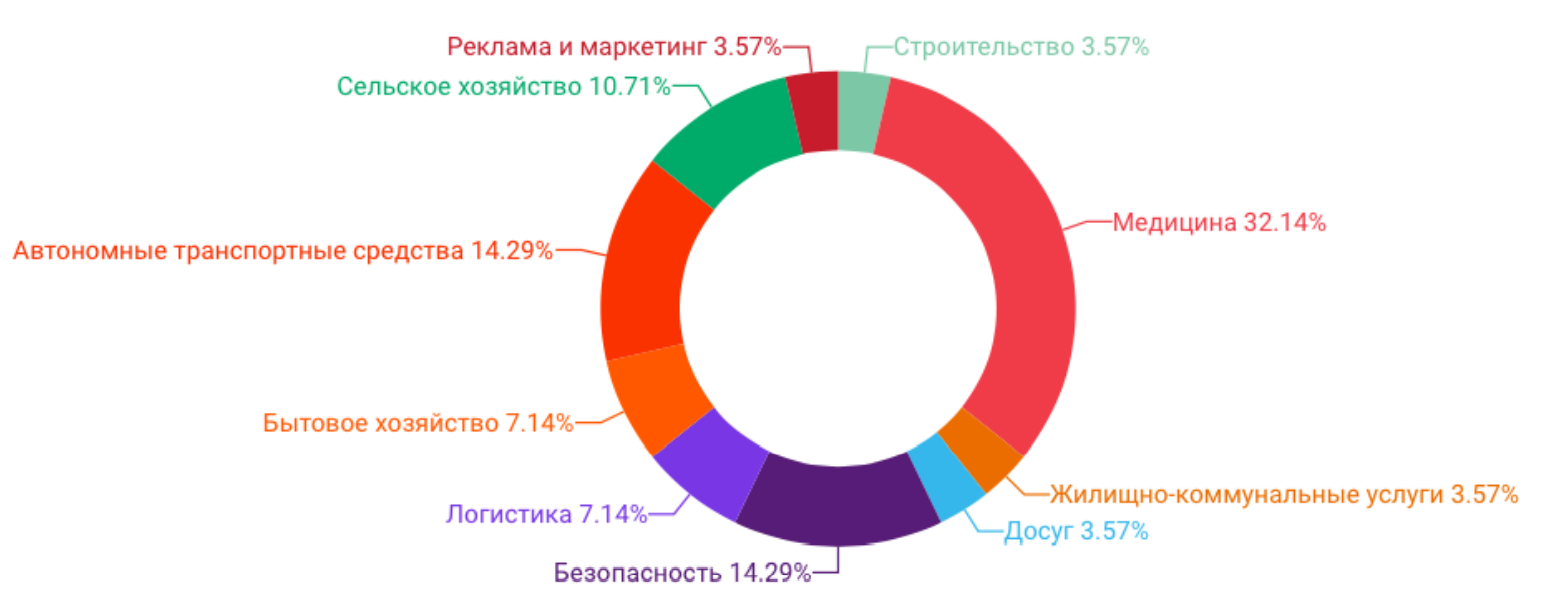
\includegraphics[width=0.9\textwidth]{Рисунки/диаграмма стата.png}
\caption{\centering \onehalfspacing {Перспективные области сервисной робототехники \cite{litlink2}}}
\label{част}
\end{center}
\end{figure}

Общий объем импорта роботизированных систем для медицинской диагностики в 2018 году составил 23,78 млн. долларов (в натуральном выражении – 16 шт.) \cite{litlink2}. Основными причинами внедрения медицинских роботизированных систем являются нехватка квалифицированного медперсонала, растущие заработные платы, рост потребности в автоматизации рутинных и монотонных процессов.Наиболее значительным фактором, способствующим росту рынка, являются общие экономические и социальные преимущества медицинской робототехники \cite{litlink3}. Кроме того, медицинская робототехника подходит для использования в гибридных операционных - одной из быстрорастущих технологий в медицинском секторе. Сдерживающий фактор - высокая стоимость закупки интегрированных роботизированных медицинских решений.

Наибольшие прибыли сконцентрированы в сегменте ассистивных хирургических комплексов (более 55\% от общего дохода мирового рынка). Наиболее популярные системы - Da Vinci и Teletap ALF-X. Используются машины для нейрохирургии, ортопедических процедур, некатетерных чрескожных и лапароскопических вмешательств, а также для управления роботизированными катетерами. Поскольку объем этих процедур велик во всем мире, предполагается, что этот сегмент сохранит свое доминирующее положение на рынке. По тепловой карте тематик публикаций в области медицинской робототехники (рисунок 1.2) можно заметить, что наиболее востребованы хирургические роботизированные системы.

\begin{figure}[!h]
\begin{center}
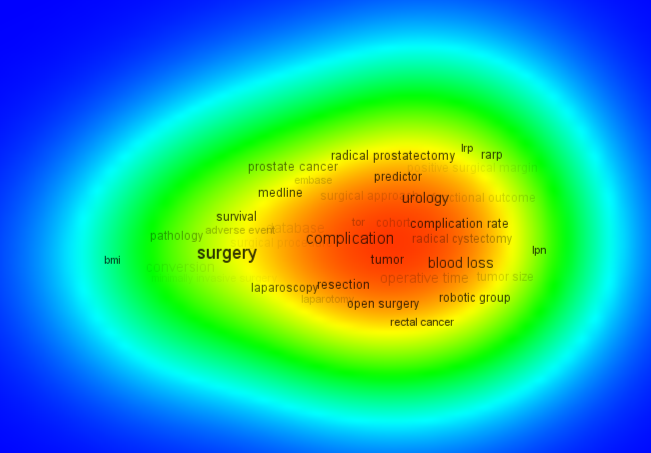
\includegraphics[width=0.7\textwidth]{Рисунки/тепловая карта.png}
\caption{\centering \onehalfspacing {Тепловая карта тематик публикаций кластера «Робототехника в медицине» \cite{litlink2}}}
\label{част}
\end{center}
\end{figure}

На ранних этапах развития возможности хирургических манипуляторов были крайне 
ограничены: не хватало вычислительных мощностей и пропускной способности каналов связи, а одной из ключевых проблем долгое время оставалась временная задержка между моментом отправки команд, производимым на операционном столе реальным хирургическим действием и итоговым получением визуального подтверждения этого действия на компьютерном мониторе. Однако рост вычислительных мощностей и пропускной способности каналов связи привели к тому, что в сентябре 2001 года была проведена первая телеуправляемая трансатлантическая операция. В этой операции использовалась первая универсальная роботизированная система Zeus, созданная в 1998 году, в состав которой входил усовершенствованный эндоскопический модуль AESOP \cite{litlink3}.

Рынок диагностического роботизированного оборудования также является крупнейшим сектором общего рынка медицинского оборудования \cite{litlink4}. Наиболее используемые роботы для медицинских систем, в том числе и для систем визуализации – коллаборативные роботы (коботы). Они состоят из манипулятора и устройства управления, в виде, например, планшета, которое формирует команды, задающие требуемые движения исполнительных органов манипулятора. В Abi Research сообщается  \cite{litlink4}, что среднегодовой прирост на рынке коботов в период с 2016 по 2025 год составит 50 \%.

Самые известные производители коллаборативных роботов — это компании Universal Robot, KUKA, Rethink Robotics и Franka. 

Медицинские роботы позволяют хирургам проводить операции более точным и менее инвазивным способом. Они используются из-за их способности выполнять повторяющиеся задачи на высоких скоростях без снижения качества из-за отсутствия фактора утомляемости. Роботизированный метод дает большие преимущества не только с точки зрения производительности, но и с точки зрения экономической эффективности. Основной целью внедрения медицинской робототехники является сокращение количество медицинских сотрудников и улучшение диагностических возможностей во время операции. 


%Существует телеультразвуковая система на базе робота французской компании AdEchoTech. Она обеспечивает возможность проводить ультразвуковое исследование под контролем обычного врача, когда эксперт в области УЗИ находится на удаленном расстоянии. В этой системе используется роботизированная рука Melody, позволяющая в реальном времени управлять удаленным от оператора датчиком и проводить диагностику.При этом система УЗИ-специалиста (Melody Expert) и система пациента (Melody Patient) работают совместно через Интернет и в реальном времени обмениваются информацией, а также обеспечивают управлением роботом. MELODY Patient очень точно повторяет движения, которые производит УЗИ-специалист. В ней используется имитатор зонда в виде копии стандартного ультразвукового датчика, с помощью которого можно контролировать движения робота издалека.Система сертифицирована FDA для использования на рынке США. И это единственная такая система.Вторая система имеет название HER (Hapticaly-Enabled Robotics) Remote Ultrasound, может применяться для исследования брюшной полости с целью оценки состояния почек, печени, желчного пузыря, поджелудочной железы, селезенки, а также брюшной аорты и других кровеносных сосудов. Система имеет встроенную технологию получения обратной связи от пациента, что позволяет специалисту дистанционно отслеживать дискомфорт пациента, связанный с силой давления УЗИ-датчика. Эта информация может использоваться для оценки чувствительности исследуемой области и для сравнения ее с данными предыдущих исследований пациента.Принципиальным преимуществом этой системы является ее способность транслировать чувство прикосновения оператора. Такая тактильная обратная связь помогает оператору ощущать удаленную среду посредством роботизированной системы. Для оценки ситуации, ощущения глубины восприятия и общения с пациентом используется система видеосвязи. Связь осуществляется посредство 4G-сети мобильной связи компании Telstra.Также аналогом является роботизированная система Tele Robotic Ultrasound for Distance или TRUDI, которая позволяет оператору проводить ультразвуковые исследования из любого места, где есть Интернет. Эта система интегрирована в роботизированный киоск, и оператор может ею управлять, манипулируя УЗИ-датчиком, легко устанавливая его в нужную позицию, что позволяет проводить исследование буквально за несколько минут.Система находится пока на ранней стадии разработки и когда она будет доведена до коммерческого уровня пока неизвестно.Для ее работы необходимо иметь телекоммуникационный канал в 4 - 5Мбит/с — это обеспечивает необходимое качество передаваемой картинки при диагностике органов брюшной полости. Для эхокардиографии и исследования сосудов требуется более широкая полоса.Наиболее известным и высокотехнологичным роботизированным хирургом можно назвать систему da Vinci. На данном этапе робот не оперирует сам, а лишь подчиняется командам врача. Последний сидит за специальной консолью и управляет машиной с помощью джойстиков и педалей. За работой он наблюдает через специальный экран, куда выводится многократно увеличенное 3D-изображение в HD-качестве.Еще один ассистент находится у самого робота и помогает переключаться между инструментами. Задачи медицинских роботов da Vinci весьма широки: с их помощью проводятся операции (в том числе сложные и/или нетипичные) на сердце, щитовидной железе, на органах таза и брюшной полости.Осенью 2017 года появилась информация, что в России готовится к промышленному производству аналогичный робот-хирург, по ряду параметров даже превосходящий da Vinci. Особенно подчеркивалось, что отечественная система позволит проводить операции удаленно – например, кардиохирург из Санкт-Петербурга сможет управлять роботом, находящимся, допустим, в Тюмени. На месте процесс будет контролировать хирург общего профиля. Такие «удаленные» системы разрабатываются и другими компаниями. Например, робот Raven из США, который, помимо прочего, обладает искусственным интеллектом и дает врачу подсказки, как можно поступить в той или иной ситуации.


\section{Области применения ультразвуковой роботизированной визуализации}

Ультразвуковое исследование стало незаменимым методом медицинской визуализации как для диагностики, так и для хирургических вмешательств. Будучи безрадиационным, портативным, широко доступным методом визуализации в режиме реального времени, он имеет значительные преимущества по сравнению с другими методами, такими как компьютерная томография (КТ) или магнитно-резонансная томография (МРТ). Кроме того, четырехмерное ультразвуковое исследование обеспечивает достаточно высокую частоту кадров для многих медицинских задач. Однако его успешное проведение сильно зависит от опыта специалиста, который должен правильно определить поле зрения, таким образом, постоянно фокусируясь на экране монитора и удерживая датчик вручную с соответствующим давлением. Врач также должен настроить несколько параметров визуализации на ультразвуковом аппарате. Этот неэргономичный процесс обследования также может привести к профессиональным заболеваниям опорно-двигательного аппарата. Кроме того, ручное управление зондом делает получение воспроизводимого изображения практически невозможным. В то время как пространственно и временно разделенное получение изображений и диагностика являются обычной практикой для МРТ и КТ, сонографы должны выполнять и то, и другое одновременно.

Роботизированное ультразвуковое исследование представляет собой сочетание роботизированной системы и ультразвукового блока с датчиком, прикрепленным к рабочему органу робота. Такая система может использоваться, например, для трекинга катетера для эндоваскулярной пластики аневризмы \cite{litlink5}. Во время вмешательства врач вводит катетер в брюшную аорту, а эндоваскулярный инструмент направляется в область интереса. Робот следует за катетером, используя алгоритм отслеживания и управления силой, так что кончик катетера постоянно виден на ультразвуковых изображениях. Также роботизированный ультразвук часто применяется при биопсии \cite{litlink6}.

Другой областью применения является лечение опухолей с помощью высокоинтенсивного фокусированного ультразвука \cite{litlink7}. Два ультразвуковых датчика 2D, установленные на датчике высокоинтенсивного фокусированного ультразвука, используются для трекинга, и система регистрирует изображения, сравнивая их с изображениями до вмешательства. Пока ультразвуковые датчики и преобразователь являются статичными, но авторы планируют использовать данную систему с двумя роботами в будущем.

В \cite{litlink8} предложено автоматизированное роботизированное выравнивание пациента под ультразвуковым контролем, чтобы свести к минимуму деформацию мягких тканей. Чтобы обеспечить точную лучевую терапию, во все дни лечения необходимо создавать одинаковые деформации мягких тканей. В этом исследовании предполагается, что аналогичные деформации мягких тканей получаются, когда их ультразвуковые изображения одинаковы. Поскольку при КТ-сканировании и лучевой терапии используется ионизирующее излучение, врач не может держать датчик на пациенте, поэтому необходима автоматизированная роботизированная система (рисунок 1.3).

\begin{figure}[!h]
\begin{center}
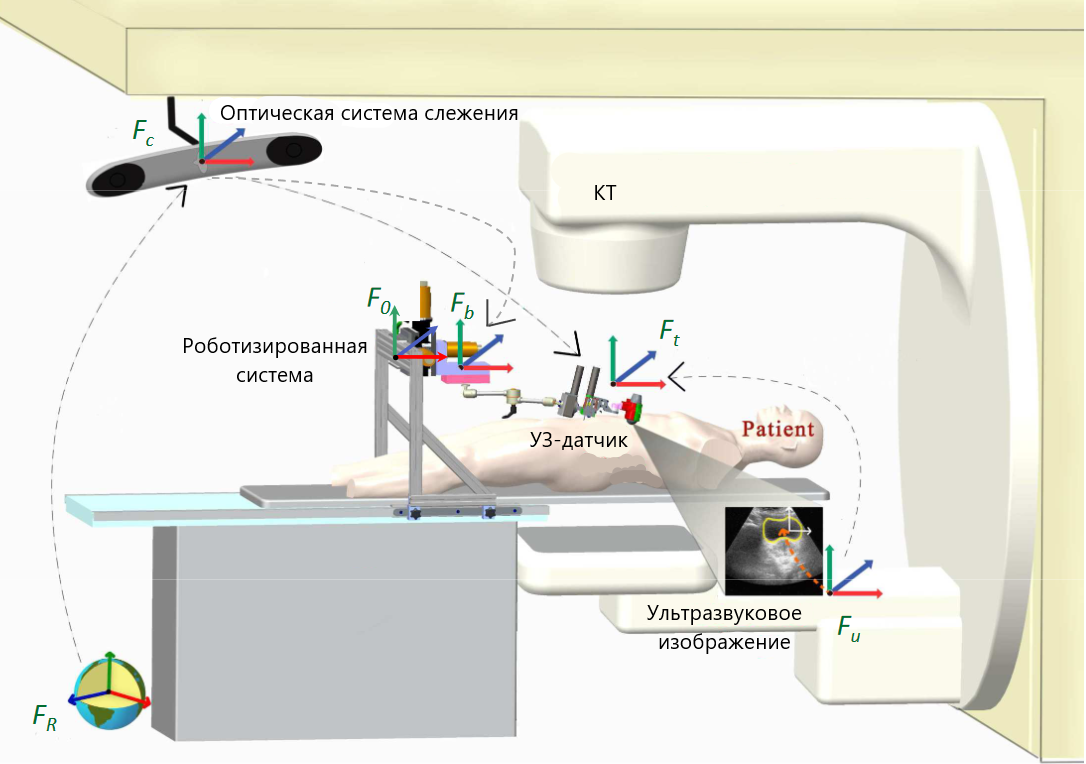
\includegraphics[width=0.7\textwidth]{Рисунки/система слежения.png}
\caption{\centering \onehalfspacing {Комплекс с роботизированной системой для проведения лучевой терапии \cite{litlink8}}}
\label{част}
\end{center}
\end{figure}

\section{Описание модели биологического объекта}

Чаще всего, доступ хирургического инструмента к сосуду осуществляется через бедренную артерию в верхней части бедра, реже — через плечевую, лучевую, подколенную и другие артерии. Поэтому объектом исследования является бедренная артерия, которая состоит из трех слоев: наружного, гладкомышечного слоя и эндотелия. На рисунке 1.4 изображены система артерий нижних конечностей и расположение бедренной артерии в ней.

\begin{figure}[!h]
\begin{center}
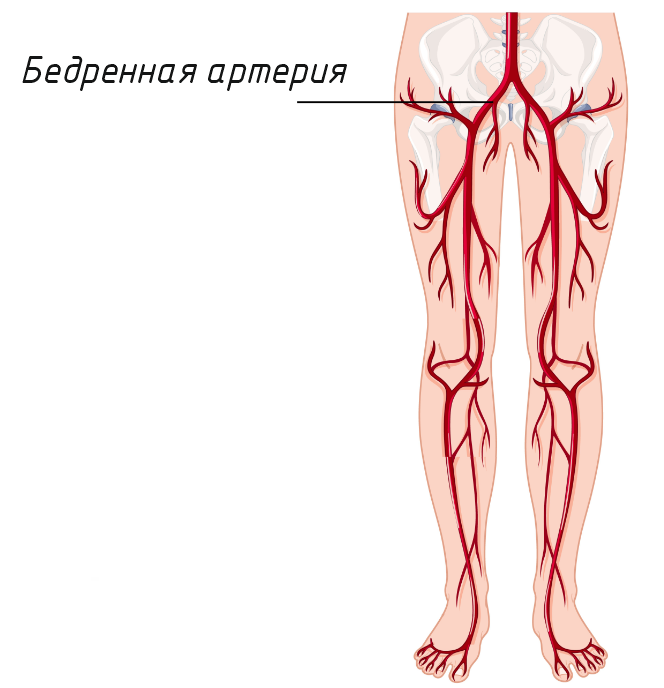
\includegraphics[width=0.4\textwidth]{Рисунки/бедренная артерия.png}
\caption{\centering \onehalfspacing {Локализация бедренной артерии в нижних конечностях}}
\label{част}
\end{center}
\end{figure}

Образование тромбов, сгустков крови в кровеносном сосуде, является самой распространенной проблемой, связанной с артериальными сосудами. Острый артериальный тромбоз является непосредственной причиной большинства случаев инфаркта миокарда (сердечного приступа) и примерно 80\% инсультов, что в совокупности является наиболее распространенной причиной смерти. На рисунке показана схема образования тромбоза в сосудистом русле \cite{litlink9}.

Первичным триггером артериального тромбоза является разрыв атеросклеротической бляшки, которая развивается за счет накопления липидных отложений и липид-нагруженных макрофагов (пенистых клеток) в стенке артерии \cite{litlink9}. Тромбы, которые образуются при разрыве бляшки, богаты тромбоцитами, которые представляют собой маленькие (около 1 мкм в диаметре) безъядерные клетки. Эти дискообразные клетки циркулируют в крови и образуют первичную гемостатическую пробку в местах повреждения сосудов. Если тромб оторвался от стенки сосуда его называют эмболой. На рисунке 1.5 схематично показано сосудистое русло артерии при нормальном кровотоке и при артериальном тромбозе.

\begin{figure}[!h]
\begin{center}
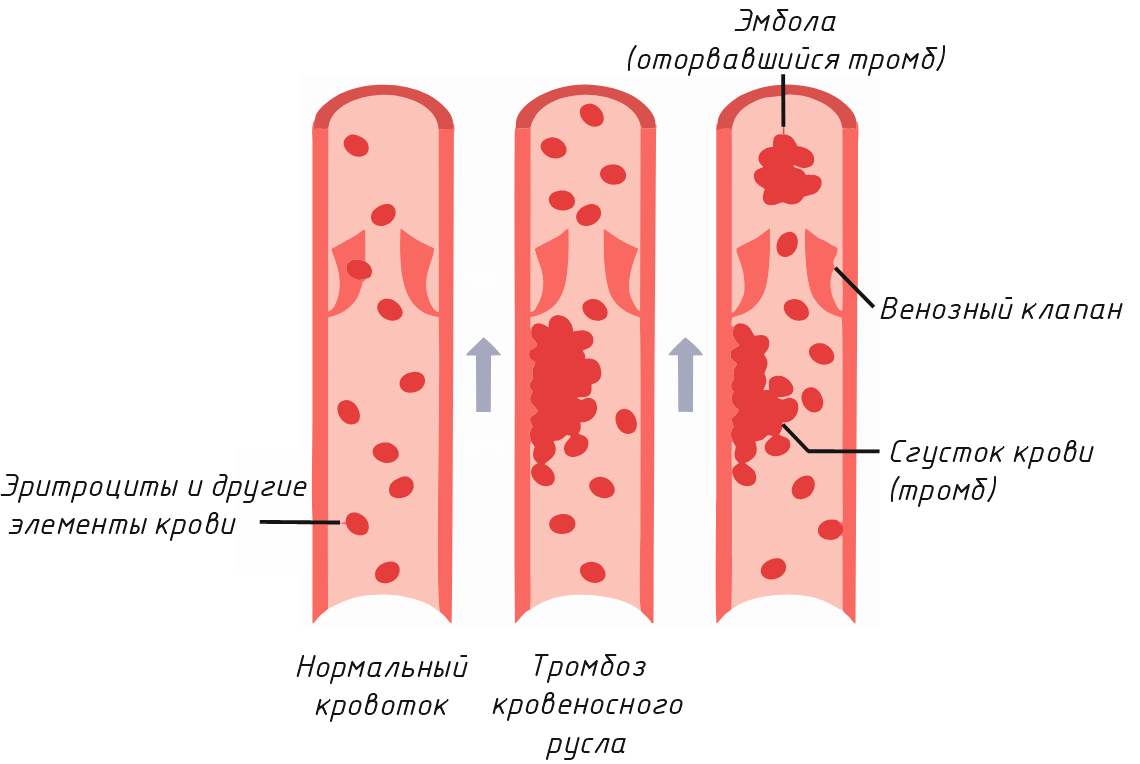
\includegraphics[width=0.8\textwidth]{Рисунки/тромбоз.png}
\caption{\centering \onehalfspacing {Сосудистое русло артерии при нормальном кровотоке и при артериальном тромбозе}}
\label{част}
\end{center}
\end{figure}

Отрыв тромбов может приводить к полной закупорке (тромбоэмболии) более мелких кровеносных сосудов. Процедуру хирургического удаления тромбов (тромбоэмболов) называют тромбоэктомией \cite{litlink10}. Оперативное вмешательство при эмболиях заключается в удалении эмбола катетером, сосудистыми кольцами, вакуум-отсосом или с помощью ретроградного промывания артерий. Наибольшую популярность среди них в последнее время получил метод эмболэктомии специальным баллонным катетером Фогарти. Его применение сделало операцию малотравматичной, простой и значительно повысило ее эффективность. Оперативные вмешательства при острых тромбозах принципиально отличаются от операций при эмболиях, они заключаются в том, что одновременно с тромбэктомией необходимо ликвидировать также причину заболевания, то есть выполнить ту или иную реконструкцию артерий \cite{litlink10}.

\section{Методы определения положения внутрисосудистых инструментов}

Диагностические и терапевтические процедуры под визуальным контролем стали обычной практикой для малоинвазивных вмешательств. Ультразвук, рентгеноскопия, магнитно-резонансная томография (МРТ) и компьютерная томография (КТ) используются для управления хирургическим инструментом во время вмешательства. Данные методы должны обеспечивать высокую точность, минимальную дозу ионизирующего облучения и доступность для использования в операционных.

\subsection{Рентгеновская визуализация}

Рентгеновская визуализация подразделяется на 4 вида: рентгенография, флюороскопия, ангиография и мультидетекторная КТ \cite{litlink11}. Все они имеют источник, детектор рентгеновского излучения и соответствующие системы управления. Каждый из этих методов, основанных на рентгеновских лучах, использует разные подвижные, как правило кольцевые, части томографического аппарата и детекторы \cite{litlink11}.

Рентгенография — исследование внутренней структуры организма, изображение которой создается при помощи рентгеновских лучей и проецируется на рентгеновскую пленку. Рентгенография позволяет рентгенологу не находиться в одной комнате с исследуемым во время включения рентгеновского аппарата и не подвергаться самому дополнительному облучению. Однако основным недостатком этого метода является невозможность оценить состояние организма при его функционировании. Рентгенограмма позволяет увидеть только функционирование в один момент времени.

Флюороскопия - это метод рентгенологического исследования, при котором изображение объекта получают на светящемся (флюоресцентном) экране. Этот метод используется для непосредственного наблюдения в режиме реального времени \cite{litlink12}. Его главное ограничение - невозможность четко визуализировать твердые органы из-за низкого пространственного разрешения. 

Ангиография - контрастное рентгенологическое исследование кровеносных сосудов, при котором в просвет сосуда вводится специальный контрастный материал и производится регистрация сигнала от контраста внешним считывающим устройством. Принцип метода состоит в том, что контрастный препарат заполняет внутренний просвет сосуда и, при наличии нарушения его проходимости, позволяет выявить область или точное место поражения сосуда.

Мультидетекторная компьютерная томография (МДКТ) отличается высокой точностью и скоростью проведения. Особенностью этого метода является то, что специальный излучатель рентгеновских лучей в томографе непрерывно вращается. МДКТ преобразует обычные аксиальные (перпендикулярные к срединной линии тела) срезы в трехмерное изображение.

Обычно эндоваскулярные вмешательства выполняются под контролем флюороскопии и цифровой субтракционной ангиографии, в основе которой лежит принцип компьютерного вычитания (субтракции) двух снимков до и после введения контрастного вещества в сосуд, чтобы визуализировать в реальном времени текущее положение хирургических инструментов \cite{litlink13}. Цифровая субтракционная ангиография используется для обеспечения правильного развертывания и положения стент-графта \cite{litlink11}.

Флюороскопия по-прежнему применяется при визуализации иглы во время биопсии легких, хотя во многих учреждениях ее использование почти полностью заменено КТ из-за ее более высокого разрешения. Она предпочтительнее, если пациент страдает ожирением \cite{litlink13}.

Благодаря быстрому получению данных, высокому разрешению, хорошей доступности и низкой стоимости, КТ является одним из лучших методов для процедур с визуальным контролем \cite{litlink14}. Из методов, основанных на рентгеновских лучах, КТ является самой востребованной из всех интервенционных процедур, требующих получения изображения поперечного сечения исследуемого объекта и широко используется для визуального контроля. Она предпочтительнее флюороскопии, МРТ и ультразвука из-за доступности, отсутствия серьезных противопоказаний, простоты использования и визуализации с высоким пространственным разрешением \cite{litlink11}.

Для повышения точности и уменьшения рентгеновского облучения при вмешательствах под контролем КТ был разработан ряд навигационных систем \cite{litlink15}. Некоторые системы были клинически протестированы в ходе сравнительных \cite{litlink16, litlink17} и рандомизированных исследований \cite{litlink18}. Эти навигационные системы включают локатор (оптический или электромагнитный), который отслеживает в реальном времени положение иглы. В статье \cite{litlink14} описаны результаты рандомизированного клинического исследования по оценке прототипа электромагнитной навигационной системы IMACTIS CT (Imactis SAS, Ла Тронш, Франция). Эта система позволяет интервенционному радиологу визуализировать запланированную траекторию движения иглы до ее введения в реальном времени (рисунок 1.6).

\begin{figure}[!h]
\begin{center}
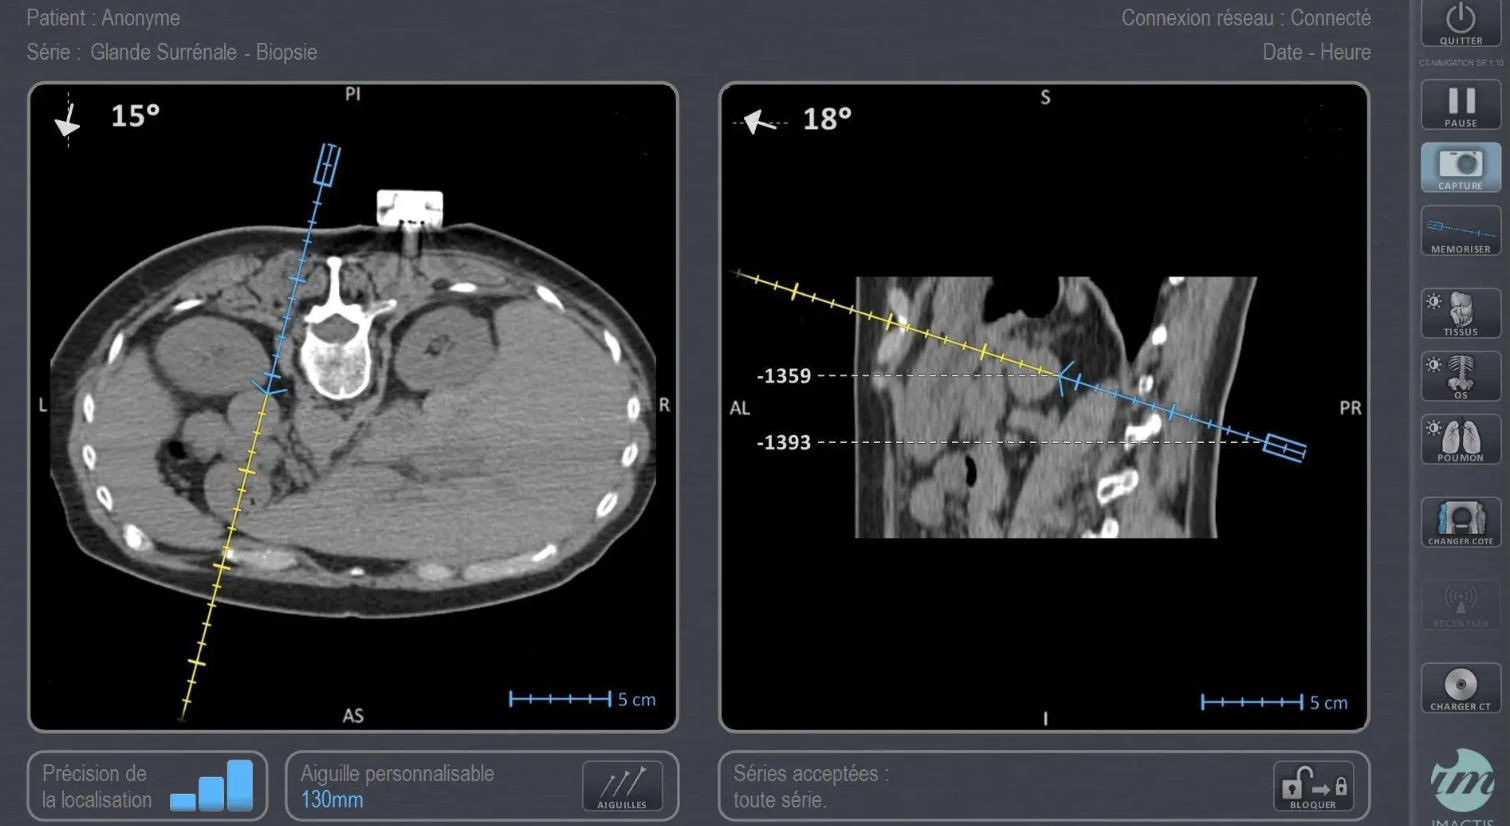
\includegraphics[width=0.8\textwidth]{Рисунки/КТ.png}
\caption{\centering \onehalfspacing {Изображение с навигационной системы IMACTIS
CT-NAVIGATION \cite{litlink14}}}
\label{част}
\end{center}
\end{figure}

Результаты исследования систем показали, что с помощью данной навигационной системы можно достичь выигрыша во времени и точности (до 4,1 мм) по сравнению со стандартным вмешательством под контролем КТ (точность до 8,9 мм).

В последнее время при хирургических вмешательствах с помощью КТ используется преимущественно настольная КТ. Томография с использованием С-образной дуги (С-дуга), которая включает в себя как источник рентгеновского излучения, так и детекторы, вращающей вокруг пациента и создающей
трехмерный набор изображений, подобных КТ (рисунок 1.7) \cite{litlink19,litlink20}.

\begin{figure}[!h]
\begin{center}
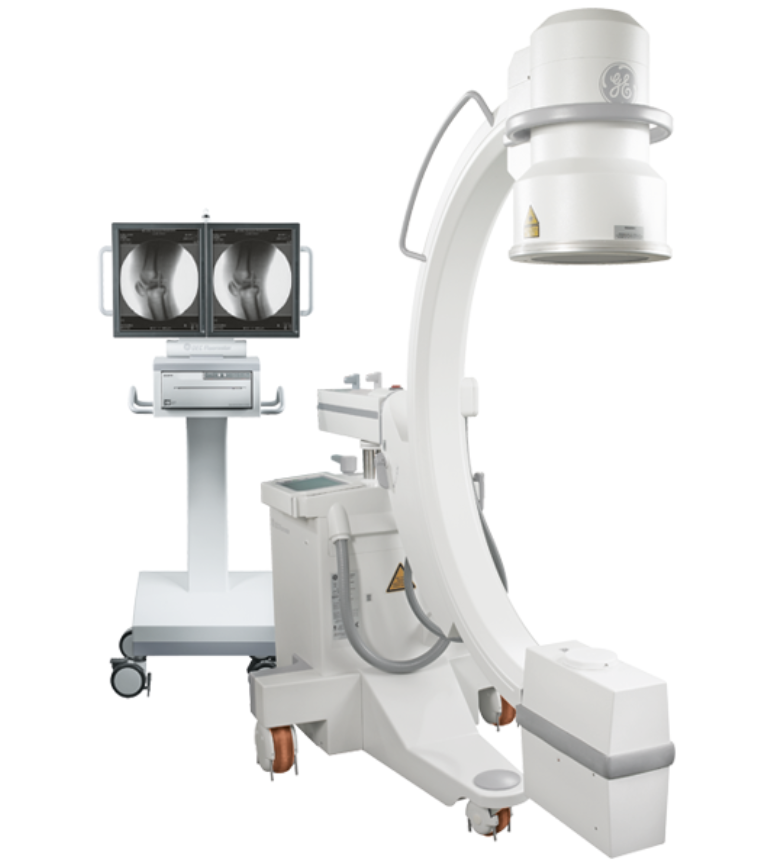
\includegraphics[width=0.5\textwidth]{Рисунки/КТ2.png}
\caption{\centering \onehalfspacing {Аппарат OEC Fluorostar Compact}}
\label{част}
\end{center}
\end{figure}

При сосудистых вмешательствах С-дуга используется для оценки относительного положения инструментов по сравнению с рассматриваемой анатомией \cite{litlink11}. Данный метод позволяет получать изображения в реальном времени с частотой кадров 25–30 кадров/с. КТ с C-дугой имеет лучшую визуализацию металлических артефактов по сравнению с традиционной КТ. Это может быть преимуществом при использовании данного метода визуализации при внутрисосудистом развертывании стента. Однако динамический диапазон получаемого изображения ограничивается 8–10 битами на пиксель (при традиционном КТ 14-16 бит на пиксель) \cite{litlink19}. Следовательно, могут быть визуализированы только высококонтрастные структуры, такие как сосуды и кости.

К недостаткам КТ относится введение йодсодержащего контрастного вещества, которое может вызвать аллергические реакции или почечную недостаточность. Кроме того, стоимость и наличие ионизирующего излучения ограничивают ее использование для длительного наблюдения. Также отсутствие контроля в реальном времени во время продвижения инструмента является серьезным недостатком. Чтобы его исключить, используются другие системы, такие как КТ-рентгеноскопия, конусно-лучевая компьютерная томография. Хотя они обеспечивают режим контроля в реальном времени, доза облучения при этом увеличивается \cite{litlink15}.

\subsection{Магнитно-резонансная томография}

Во многих медицинских центрах по всему миру проводятся эндоваскулярные процедуры под контролем МРТ. Высокий потенциал эндоваскулярной интервенционной МРТ объясняется тем, что она сочетает в себе трехмерную анатомическую визуализацию и определение локализации хирургического инструмента. Однако недостатками являются высокая стоимость томографа и акустический шум во время визуализации \cite{litlink21}. 

МРТ предоставляет анатомическую информацию о ткани-мишени с меньшим пространственным и временным разрешением по сравнению с рентгенографией. Интраоперационная МРТ дает возможность коррекции навигационных данных по ходу операции и повышает качество хирургического вмешательства, однако требует специального оборудования операционной, немагнитных аппаратов и инструментов. Низкопольные портативные МР-томографы требуют большего времени сканирования из-за низкой разрешающей способности, что увеличивает время операции и не позволяет проводить дополнительные исследования кровотока по ходу операции \cite{litlink22}.

Диагностические МРТ-сканеры высокого поля (от 1,0 до 1,5 Тл) не предназначены для интервенционного использования \cite{litlink23}. Было разработано несколько открытых интервенционных МРТ-сканеров с низким полем (от 0,064 до 0,5 Тл), но временное и пространственное разрешение, достигаемое с помощью таких сканеров, недостаточно для проведения эндоваскулярных процедур или получения точной функциональной информации.

Для отслеживания эндоваскулярных устройств было предложено несколько методов (рисунок 1.8).

\begin{figure}[!h]
\begin{center}
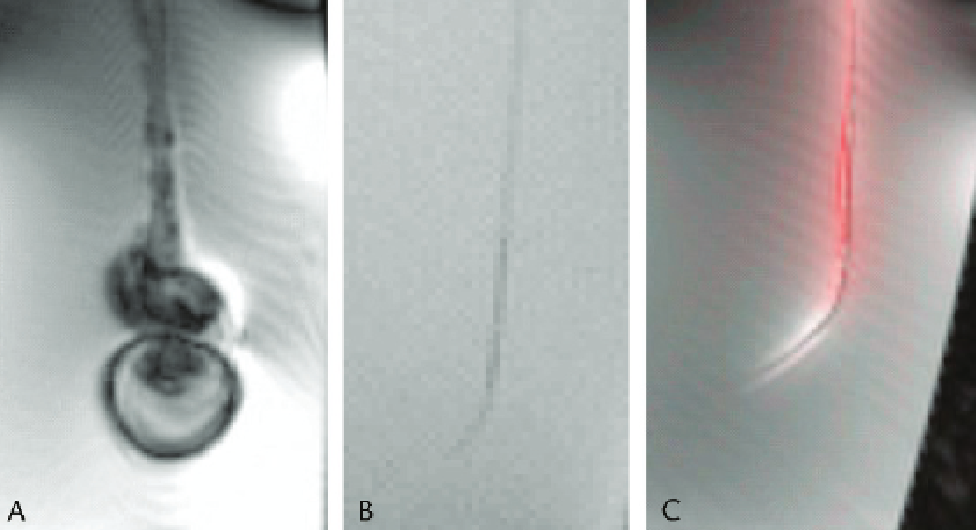
\includegraphics[width=0.8\textwidth]{Рисунки/МРТ.png}
\caption{\centering \onehalfspacing {Изображения катетеров различных конструкций для эндоваскулярных вмешательств под МРТ. A - пассивный рентгеновский
катетер с оплеткой из нержавеющей стали, вызывающий значительные
артефакты изображения. B - тот же катетер без стальной оплетки, что
делает его почти незаметным на изображении. C - активный катетер c
приемной катушкой \cite{litlink21}}}
\label{част}
\end{center}
\end{figure}

В так называемом «пассивном подходе» катетеры изготавливают из ферромагнитных материалов, чтобы увеличить их контраст на изображении \cite{litlink24}. Такие методы визуализации применяются при биопсии, а также подходят для вмешательств с использованием катетера. В отличие от жестких прямых биопсийных игл, которые можно полностью визуализировать на одном изображении, полученном вдоль стержня иглы, ангиографические катетеры гораздо более гибкие, что позволяет им повторять форму сосудов внутри человеческого тела. Следовательно, невозможно визуализировать весь ангиографический катетер с помощью метода визуализации, основанного на одном срезе. Хотя кончик катетера является основной целью для отслеживания, весь катетер должен постоянно визуализироваться во время вмешательства.

Другой подход к визуализации инструмента заключается в использовании проволоки в качестве приемной катушки. В «активном подходе» радиочастотные сигналы принимаются одной или несколькими микрокатушками \cite{litlink24}, встроенными в интервенционное устройство. Схема настроена на частоту МРТ-сканера. Эти сигналы отправляются в один из каналов приемника системы МРТ, где они оцифровываются и затем используются для определения положения катушки приемника в магните. Положение катушки может отображаться у оператора в виде курсора, наложенного на предварительно полученное статическое изображение.

В рамках исследования \cite{litlink25} была разработана и изготовлена двухэлементная катетерная фазированная (с электронным сканированием) матрица для активного отслеживания и визуализации стенок сосудов с высоким разрешением. Продвижение и втягивание катетера было успешно отслежено как в экспериментах с фантомом сосудов, так и в экспериментах по визуализации на свиньях. Отслеживание инструмента (местоположение и ориентация) были признаны работающими очень надежно и точно в более чем 1000 кадрах отслеживания/визуализации. Успешная локализация определялась, когда центр среза был размещен в пределах 2 мм от катушек слежения, а ориентация среза содержала в себе обе соленоидные катушки. Измеренная частота успеха составила 100\% для неподвижного катетера и > 97\% для движущегося катетера со скоростью до 3 см/с в аорте. В экспериментах с фантомом in vivo точность смещения оказалась больше, чем 2 мм, а точность ориентации среза больше, чем 2°. На изображениях стенки сосуда разрешение 240 мкм было достигнуто при времени экспозиции 15 с/срез. Артефактов, ухудшающих внешний вид стенки сосуда, не наблюдалось. По сравнению с рентгеновской визуализацией, которая обычно использует изображения с разрешением 1024x1024 пикселя при 15 кадрах в секунду, типичное интервенционное МР-изображение будет составлять 192x128 пикселей при 8 кадрах в секунду \cite{litlink21}.

\subsection{Электромагнитная навигация}

С-дуги обеспечивают только 2D-проекцию, и, как следствие, отсутствие
восприятия глубины затрудняет визуальную оценку положения и ориентации
катетеров внутри сосудистой сети пациента \cite{litlink26}. Кроме того, во время процедуры врач должен выполнить несколько измерений и корректировок положения и ориентации С-образной дуги: плохие углы проецирования могут вызвать такие проблемы, как ложное сужение сосудов и обскурация (затемнение) сосудов из-за перекрывающих сосудов или костей. Кроме того, традиционными катетерами трудно управлять и контролировать, и, следовательно, существует риск таких осложнений, как расслоение или перфорация сосудов \cite{litlink26}.

Принцип действия систем электромагнитной навигации основан на том,
что специальный генератор (работающий на постоянном или переменном токе) создает вокруг пациента электромагнитное поле, являющееся системой координат, в котором находится хирургический инструмент, оснащенный встроенным электромагнитным сенсором, либо на котором зафиксирован специальный адаптер. Перемещение сенсора в пространстве изменяет характеристики поля в этой точке, что позволяет навигационной системе определять координаты инструмента. В исследовании \cite{litlink26} безрамной электромагнитной навигации была описана система, которая позволила отслеживать угол наклона и ориентацию в пространстве хирургического инструмента с установленным на нем электромагнитным сенсором с погрешностью в пределах 4 мм.

Была предложена компьютерная хирургическая навигационная система, способная объединить объемную информацию, извлеченную из данных 3D-ангиографии, с электромагнитным отслеживанием в реальном времени эндоваскулярных инструментов: таким образом, хирург может следить за движением катетеров внутри трехмерной модели сосудистой сети пациента, не требуя получения флюороскопических изображений в реальном времени.

Максимальная такой визуализирующей системы составила 1,7 мм за серию из 70 измерений и средняя погрешность 1, 2 ± 0, 3 мм. Эти ошибки связаны с точностью калибровки проводника, точностью процедуры калибровки С-образной дуги и точностью локализации электромагнитной системы внутри операционной. Точность электромагнитных датчиков с пятью степенями свободы составляет 0,9 мм. Полученную точность можно считать достаточной для канюлирования большей части висцеральных ветвей брюшной аорты, которые у взрослых имеют средний диаметр в два раза больше, чем максимальная ошибка (т.е. чревная артерия 6, 4 ± 1, 1 мм, верхняя брыжеечная артерия 7, 3 ± 1, 4 мм, правая почечная артерия 5, 2 ± 1, 3 мм, левая почечная артерия 5, 1 ± 1, 0 мм).

На рынке представлена еще одна система электромагнитного трекинга Aurora (рисунок 1.9), создающая электромагнитное поле, в котором отслеживаются электромагнитные микродатчики. Она обеспечивает беспрепятственный трекинг датчиков, которые могут быть встроены в жесткие и гибкие медицинские инструменты, такие как ультразвуковые датчики, эндоскопы, катетеры \cite{litlink27}.

\begin{figure}[!h]
\begin{center}
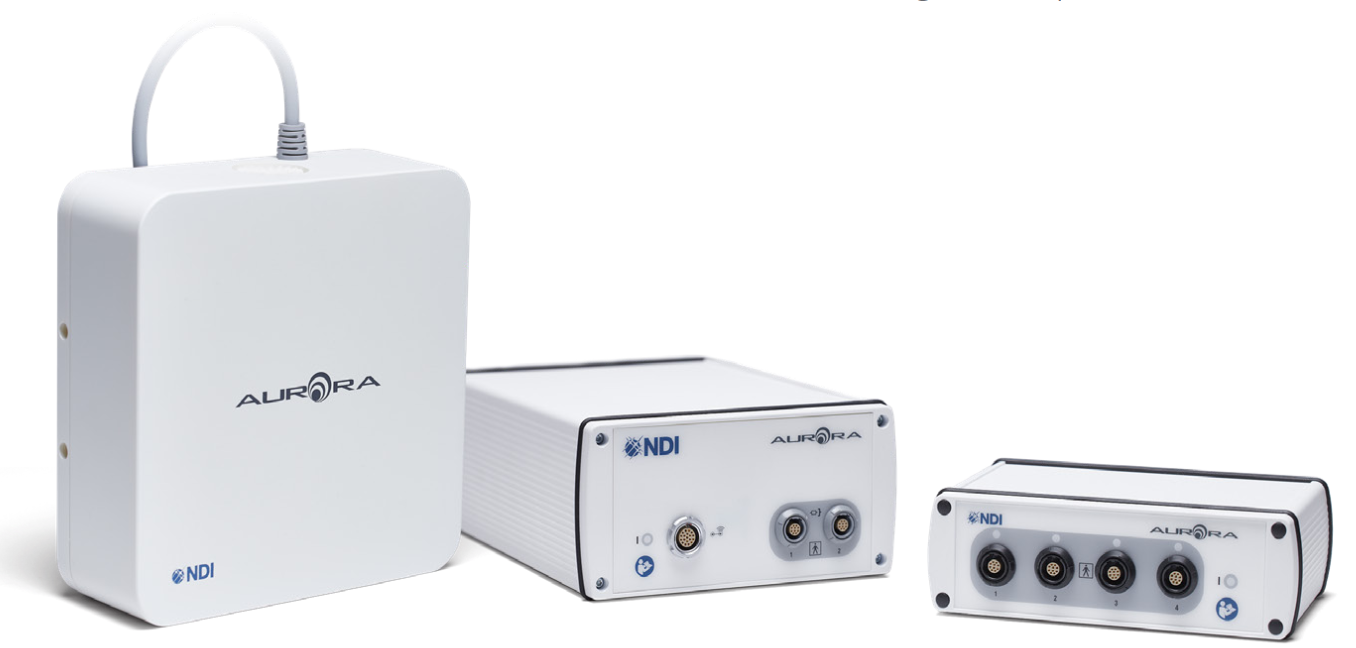
\includegraphics[width=0.8\textwidth]{Рисунки/Аврора.png}
\caption{\centering \onehalfspacing {Электромагнитная система трекинга Aurora \cite{litlink27}}}
\label{част}
\end{center}
\end{figure}

Непрерывное электромагнитное отслеживание инструментов может свести к минимуму потребность в интраоперационной рентгеноскопии, что может повысить безопасность и эффективность операции.

\subsection{Ультразвуковое исследование (УЗИ)}

Ультразвук распространенный метод трекинга инструмента при минимально инвазивных вмешательствах благодаря своей портативности и безопасности \cite{litlink28}. Основным его преимуществом перед другими передовыми методами визуализации (МРТ, компьютерная томографическая ангиография) является мобильность и работа в режиме реального времени \cite{litlink29}. Учитывая большее поле зрения, обеспечиваемое трехмерной визуализацией в реальном времени по сравнению с традиционной двумерной визуализацией, могут быть возможны более сложные процедуры под ультразвуковым контролем \cite{litlink30}. Особый интерес представляют процедуры, при которых хирургические инструменты и тканевые структуры визуализируются одновременно для достижения точных манипуляций.

Для медицинской диагностики УЗИ визуализация имеет хорошее разрешение для мягких тканей, портативность и применимость в широком диапазоне клинических условий с минимальными затратами. С помощью современных систем УЗИ возможно одновременно визуализировать жесткий наконечник инструмента (например, биопсийная игла), который направлен к удаленной цели, и саму цель \cite{litlink31}. Они включают в себя интегрирование 2D-УЗИ изображений в 3D-операционную систему с дополненной реальностью \cite{litlink32}, добавление устройства магнитного слежения к двумерному ультразвуковому датчику для предоставления дополнительных навигационных сигналов \cite{litlink33}, использование роботизированной руки для компьютерного позиционирования
биопсийной иглы под контролем УЗИ \cite{litlink34}. УЗИ предпочтительнее использовать из-за высокой частоты кадров и отсутствия излучения.

\section{Методы трекинга внутрисосудистых инструментов на изображениях с ультразвуковых визуализационных систем}

Оптическое отслеживание обеспечивает высокую точность, но требует
наличия прямой видимости между оптическими датчиками и камерой отслеживания. В результате все отслеживание положения инструмента должно выполняться снаружи. В этом случае ошибки отслеживания ориентации инструмента приводят к неверному определению положения наконечника инструмента \cite{litlink30}.

Известно, что сложные хирургические задачи с использованием двух инструментов, невозможные с 2D-контролем УЗИ, могут быть выполнены с помощью 3D УЗИ-визуализации в реальном времени с результатами, сопоставимыми с результатами, полученными с помощью оптических изображений. Для получения ультразвуковых изображений выбранной области интереса датчик необходимо расположить перпендикулярно поверхности \cite{litlink35}. 

Точка введения инструмента и траектория рассчитываются с учетом того, что ультразвуковой датчик расположен перпендикулярно поверхности пациента, а инструмент и цель находятся в одной плоскости. Из соображений безопасности инструмент может проходить только через ткань, которая уже была визуализирована.

Планирование траектории осуществляется путем проецирования области интереса на поверхность пациента. Перед получением УЗ-изображения оператор наносит достаточное количество ультразвукового геля для достижения акустической связи. Затем двумерные ультразвуковые изображения записываются одновременно с данными механического отслеживания, предоставляемыми роботизированной системой. После того, как данные записаны, изображения обрабатывают с помощью четырехсторонней интерполяции, добиваясь компромисса между вычислительной производительностью и качеством изображения.

Проблемой ультразвуковой визуализации является плохая видимость инструмента вследствие существенной разницы как в импедансе и абсорбции между биологическими тканями и инструментами, что приводит к разнообразным артефактам изображения \cite{litlink36}. С точки зрения их влияния на изображение, артефакты можно сгруппировать в три типа: артефакты сглаживания формы, в которых не видны детали формы инструмента, артефакты выпадения, в которых части инструмента появляются и исчезают при его перемещении, и топологические артефакты, изменяющие форму инструмента. Эти три типа артефактов в совокупности скрывают как геометрические детали инструмента, так и его относительное расположение относительно ткани.

В так называемом активном отслеживании применяются датчики для
определения положения инструмента с использованием ультразвукового изображения \cite{litlink30}. Приемник ультразвука, который установлен на катетере для определения интенсивности и направления ультразвукового луча, показывает положение катетера на изображении \cite{litlink37}. С помощью этого метода достигнута допустимая точность в экспериментах in vitro с различными расстояниями между катетером и ультразвуковым преобразователем, однако для определения ориентации инструмента требуется несколько электромагнитных датчиков.

В работе \cite{litlink38} представлена методика, способная обнаруживать инструменты, используемые в минимально инвазивных процедурах, такие как эндоскопические захваты, катетеры, режущие устройства. Инструменты, используемые при минимально инвазивных процедурах, имеют цилиндрическую форму и обычно диаметром 3–10 мм. Первый шаг - определить ось инструмента, для используются преобразования Радона (рисунок 1.10) \cite{litlink38}. Математическая запись преобразования Радона показана в формуле 1.1.

\begin{figure}[!h]
\begin{center}
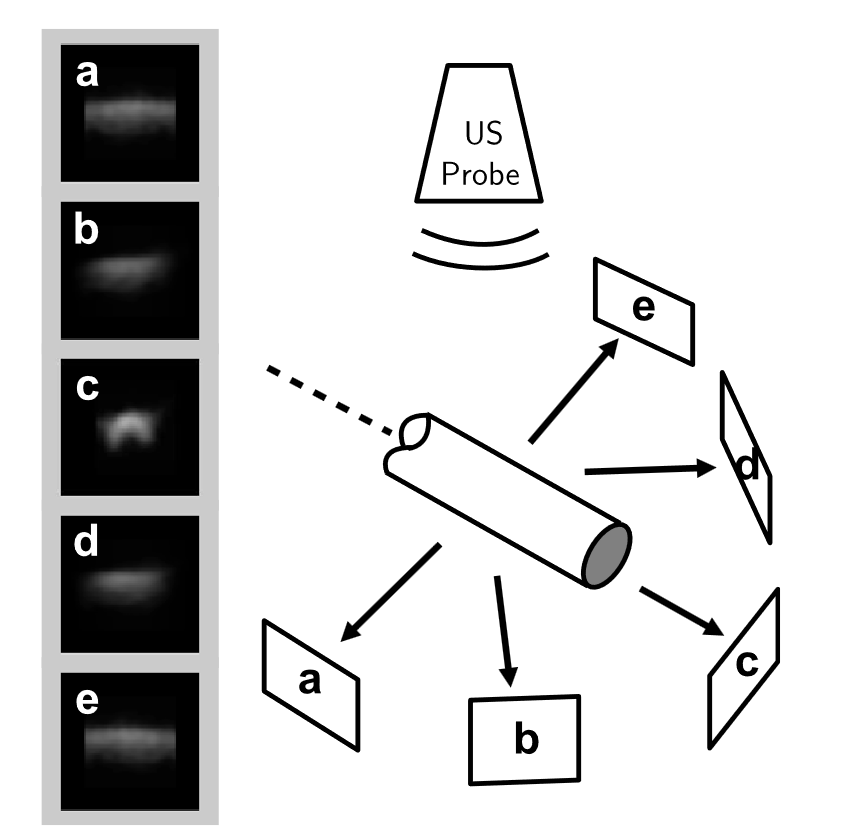
\includegraphics[width=0.5\textwidth]{Рисунки/трэкинг.png}
\caption{\centering \onehalfspacing {Обнаружение оси инструмента с помощью преобразования Радона. Каждое изображение (a – e) представляет собой проекцию
ультразвукового изображения в соответствующем направлении,
показанном на схеме. Проекция по оси инструмента (c) самая яркая}}
\label{част}
\end{center}
\end{figure}

\begin{equation}
\check{g}(\theta, \phi, u, v)=\int g(s \tau(\theta, \phi)+u \alpha(\theta, \phi)+v \beta(\theta, \phi)) d s
\end{equation}

где $\check{g}$ - модифицированное радоновое пространство ультразвукового объема g. Каждая точка в $\check{g}$ соответствует интегралу по трехмерной линии, определяемой четырьмя параметрами $\theta$, $\phi$, $v$ и $u$. Угловые параметры $\theta$ и $\phi$ (рисунок 1.11) \cite{litlink38} определяют ортонормированный базис, состоящий из $\alpha$, $\beta$ и $\tau$, который определяются как:

\begin{equation}
\tau=\left(\begin{array}{c}
\cos \theta \cos \phi \\
\sin \theta \cos \phi \\
\sin \phi
\end{array}\right), \alpha=\left(\begin{array}{c}
-\sin \theta \\
\cos \theta \\
0
\end{array}\right), \beta=\left(\begin{array}{c}
-\cos \theta \sin \phi \\
-\sin \theta \sin \phi \\
\cos \theta
\end{array}\right)
\end{equation}

\begin{figure}[!h]
\begin{center}
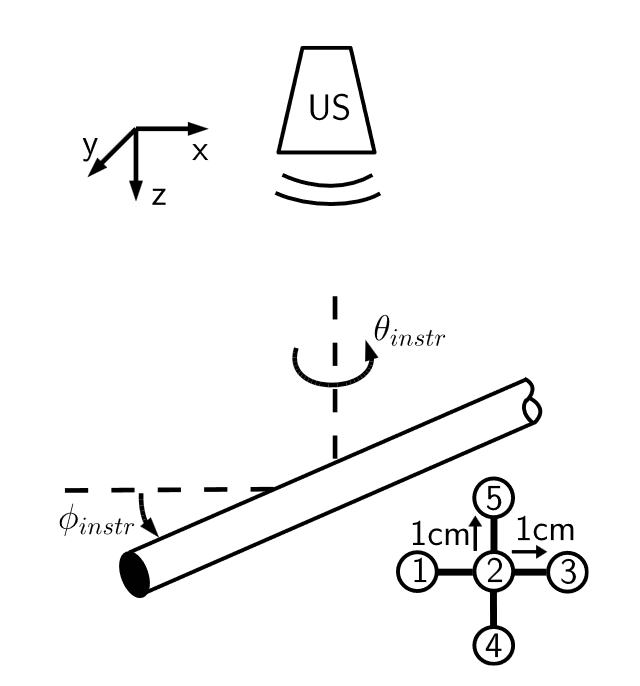
\includegraphics[width=0.5\textwidth]{Рисунки/угловые.png}
\caption{\centering \onehalfspacing {Параметры положения инструмента}}
\label{част}
\end{center}
\end{figure}

Два позиционных параметра $u$ и $v$ также используются для определения трехмерной линии. Идентификация линий в трехмерном объеме является проблемой поиска локальных максимумов $\check{g}$. При нахождении максимального значения $\check{g}$ ось инструмента в трехмерном пространстве неявно определяется параметрами ($\theta$, $\phi$, $v$ и $u$). Этот алгоритм особенно хорошо подходит для реализации в параллельных архитектурах, таких как современные графические процессоры. В первоначальной реализации он обнаруживал инструменты на ультразвуковых изображениях за 0,6 с. Чтобы улучшить эту реализацию, был усовершенствован алгоритм поиска, который определяет максимумы уравнения 1.1.

Пространство $g$ дискретизируется с шагом 5 вокселей по x, y и z. Для углов $\theta$ и $\phi$ оно дискретизируется с шагом 10 градусов. Из-за симметрии углы выбираются только от 0 до 180 градусов. Эта процедура представляет собой инициализацию отслеживания инструмента, так как поиск инструмента выполняется по всему объему. Для объемов вокселей 148x48x208 это приводит к 408 000 итерациям уравнения 1.1. Для последующих кадров алгоритм отслеживания ограничивает пространство поиска областью с центром в местоположении, найденном в предыдущем кадре. Поскольку ультразвуковые изображения обновляются с частотой 25–28 Гц, это пространство поиска может быть довольно небольшим.

В экспериментах обнаружено, что ограничение пространства поиска до ±5 вокселей в направлениях x, y и z и ± 10 градусов вокруг углов $\theta$ и $\phi$ (рисунок 1.11), найденных в предыдущем кадре, достаточно для захвата типичных хирургических движений. После того, как $\check{g}$ будет отобран в достаточной степени, максимум определяет положение оси инструмента.

\section{Сравнительный анализ существующих роботизированных систем c хирургическим и визуализирующим манипуляторами}

При проектировании роботизированной конструкции для ультразвуковой визуализации необходимо учитывать несколько параметров: минимальное рабочее пространство, точность перемещения датчика, легкая конструкция (менее 3 кг, которую может выдержать пациент), компактность робота для облегчения обследования и транспортировки \cite{litlink39}. Системы с двумя роботами-манипуляторами обеспечивают лучшую гибкость, чем системы с одним роботом, но их настройка сложнее в реализации.

Ronna G4  — роботизированная нейронавигационная система на основе шарнирных роботов-манипуляторов, предназначенная для минимально инвазивных стереотаксических процедур, таких как биопсия, стереоэлектроэнцефалография, хирургия эпилепсии и резекция опухолей (рисунок 1.12) \cite{litlink40}. Ronna может быть сконфигурирована как система с одним манипулятором, так и с двумя: одноплечевая система предназначена для стереотаксической нейронавигации и служит помощником хирурга в навигации, а двухплечевая конфигурация выполняет автономные инвазивные операционные задачи, такие как сверление кости, введение зонда или иглы и т.д. 

\begin{figure}[!h]
\begin{center}
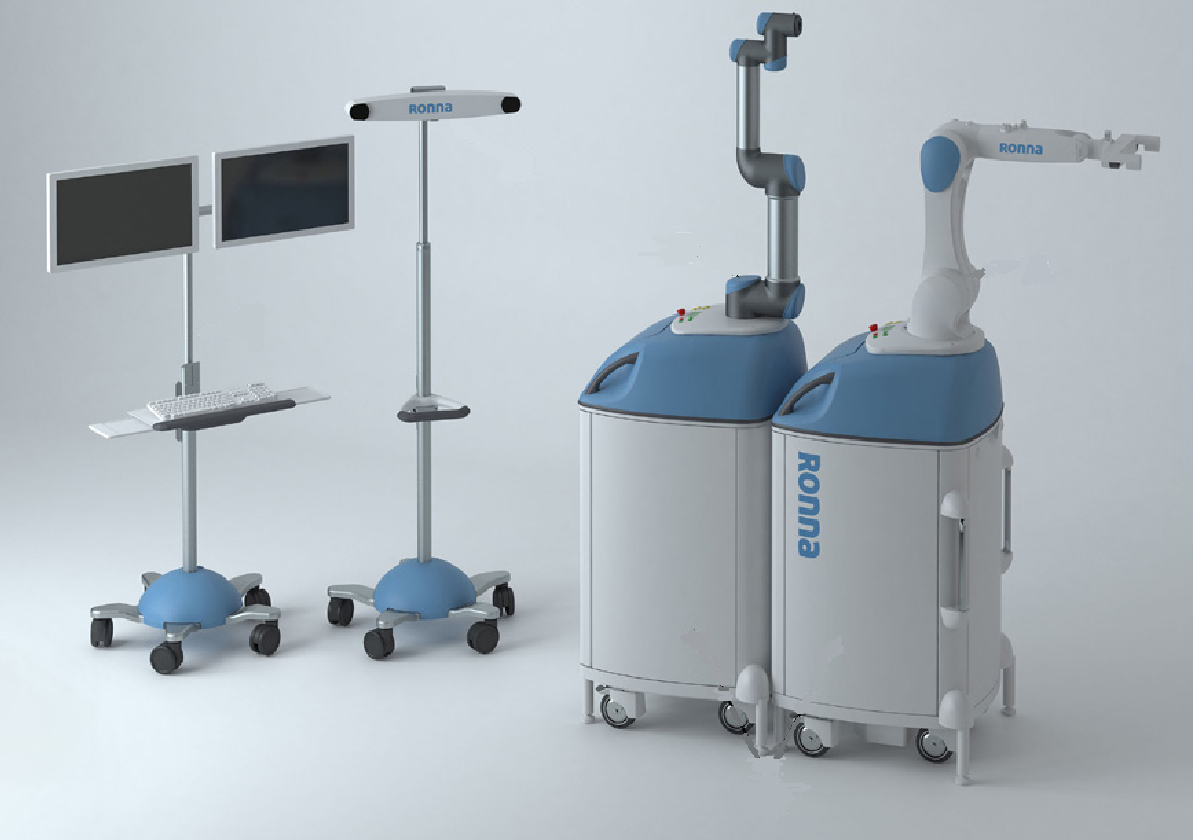
\includegraphics[width=0.7\textwidth]{Рисунки/RONNA G4.png}
\caption{\centering \onehalfspacing {Роботизированная нейронавигационная система Ronna G4 \cite{litlink40}}}
\label{част}
\end{center}
\end{figure}

Визуализирующий манипулятор управляет двумя инфракрасными камерами с макрообъективами, расположенными под углом 55° в одной плоскости. Хирургический манипулятор предназначен для автоматизированного роботизированного сверления костей и манипуляции хирургическими инструментами. Он устанавливает операционный инструмент в направляющую инструмента, указывая на рабочую точку.

Ronna обладает автоматизированным планированием положения робота и точным наведением инструмента. Система обеспечивает позиционирование хирургического инструмента во внутричерепном пространстве пациента. С 2016 года система проходит клинические испытания в университетской клинике Хорватии.

Для задач по введению иглы, таких как биопсия, предложена автоматизированная система с двумя роботами \cite{litlink35}. Система может выполнять как ультразвуковую визуализацию, так и хирургическое вмешательство. В ней используются два робота Kuka LBR iiwa, один из которых держит иглу, а другой — ультразвуковой датчик (рисунок 1.13). Визуализирующий робот позволяет контролировать силу прижатия датчика. Данные прединтервенционного планирования регистрируются в системе координат робота на этапе инициализации с использованием регистрации изображений. Врач выбирает область интереса на изображениях поверхности пациентов, полученных с помощью RGB-камер, установленных на роботах. Роботы перемещают ультразвуковой датчик и иглу в область интереса и начинают отслеживание цели на основе предварительно определенной цели, а также отслеживание иглы для введения иглы в соответствии с планом. Данная система была испытана на фантоме из желатина.

\begin{figure}[!h]
\begin{center}
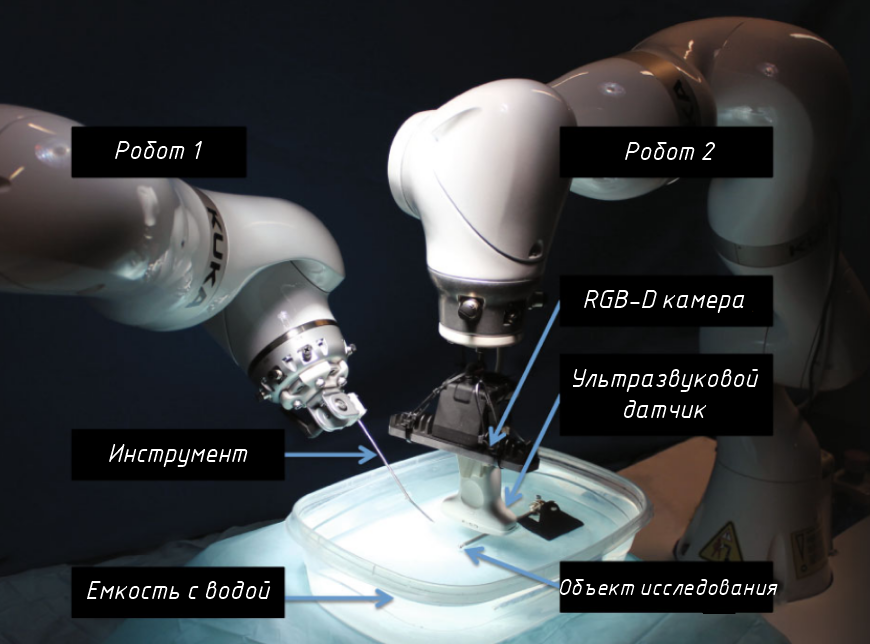
\includegraphics[width=0.7\textwidth]{Рисунки/аналог1.png}
\caption{\centering \onehalfspacing {Манипуляторы Kuka LBR iiwa, удерживающие инструмент и ультразвуковой датчик \cite{litlink41}}}
\label{част}
\end{center}
\end{figure}
\newpage

В исследовании \cite{litlink41} была разработана система для введения гибких игл под ультразвуковым контролем (рисунок 1.14). Основное преимущество данной системы заключается в том, что иглу можно точно направить к цели без необходимости выполнять многократные повторные введения, что сокращает продолжительность вмешательства. Для проведения экспериментов была использована гибкая игла со скошенным концом, прикрепленная к концевому эффектору робота Viper S650 с 6 степенями свободы (Adept Technology Inc., США). Иглу вводилась в самодельный желатиновый фантом, имитирующий мягкие ткани. Ультразвуковой контроль производится с помощью ультразвукового датчика 4DC7-3/40 3D (Ultrasonix Medical Corporation, Канада), который находится в неподвижном состоянии.   Обработка изображений выполняется на рабочей станции (Intel Core i7, NVIDIA Quadro K2000), которая получает данные от ультразвуковой системы SonixTouch и обеспечивает связь с роботом. В результате врачу отображаются два ортогональных среза, на которых выделено текущее положение иглы.

\begin{figure}[!h]
\begin{center}
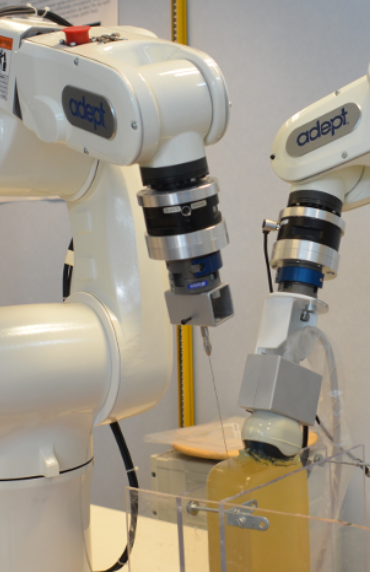
\includegraphics[width=0.4\textwidth]{Рисунки/аналог3.png}
\caption{\centering \onehalfspacing {Система из двух манипуляторов Viper S650 (Adept): хирургическим с гибкой иглой и визуализирующим с ультразвуковым датчиком}}
\label{част}
\end{center}
\end{figure}

В исследовании \cite{litlink42} создан прототип, состоящих из двух манипуляторов с шестью степенями свободы для проведения почечной пункции (рисунок 1.15). Один манипулятор выполняет ультразвуковое сканирование, другой - почечную пункцию. Оба робота-манипулятора имеют функцию позиционирования и функцию управления. Перед началом операции врач размещает два манипулятора у почки пациента и точки входа иглы. 

Сообщается, что испытания на животных подтверждают эффективность прототипа системы.
В будущем такая роботизированная система пункции может быть использована для клинических испытаний, что, как ожидается, позволит лучше контролировать смещение почек, вызванное дыханием в процессе пункции. Это повысит успешность пункционной хирургии и снизит частоту осложнений, поэтому система имеет хорошие перспективы для применения.

\begin{figure}[!h]
\begin{center}
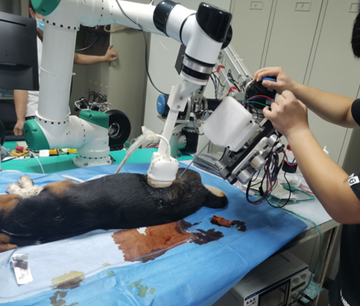
\includegraphics[width=0.6\textwidth]{Рисунки/аналог4.png}
\caption{\centering \onehalfspacing {Прототип роботизированной системы \cite{litlink42}}}
\label{част}
\end{center}
\end{figure}
\newpage

\section{Обзор существующих материалов для изготовления фантома мягких тканей}

Ультразвуковые фантомы - это неоднородные среды с определенными геометрическими и механическими характеристиками, которые используются для настройки ультразвукового оборудования. Основная часть фантома представляет собой однородное вещество с акустическими свойствами, соответствующими свойствам тканей человека с точки зрения скорости звука:

\begin{equation}
\boldsymbol{c}=\sqrt{\frac{{E}}{{\rho}}},
\end{equation}

где ${E}$ - модуль Юнга;

$\rho$ - плотность вещества.

А также затухания (дБ/см):

\begin{equation}
\boldsymbol{\alpha}=\frac{-ln (A_{d}/A_{0})}{d},
\end{equation}

где $A_{0}$ и $A_{d}$ - амплитуды звуковых колебаний до прохождения через вещество и после соответственно;

$d$ - толщина образца.

Коэффициент затухания, измеряемый в дБ/(см*МГц), рассчитывается по формуле:

\begin{equation}
\boldsymbol{\alpha_{k}}=\frac{\boldsymbol{\alpha}}{f},
\end{equation}

где f - частота ультразвукового импульса.

Последний можно модифицировать, варьируя концентрацию мельчайших включений с различными реологическими свойствами \cite{litlink43}.

В исследовании \cite{litlink44} рекомендуется использовать фантомы со скоростью звука 1540 м/с и с коэффициентом затухания 0,5-0,7 дБ/(см*МГц) для частотного диапазона от 2 до 15 МГц. 

Мягкие ткани состоят из мышц, сухожилий, связок, фасций, жира, фиброзной ткани, синовиальных оболочек, нервов и кровеносных сосудов. В таблице 1.1 указаны наиболее характерные акустические свойства мягких тканей организма.

\begin{table}[h]
\captionsetup[table]{singlelinecheck=false,justification=raggedleft}
\ttabbox
{\caption {\onehalfspacing Диапазон значений акустических свойств мягких биологических тканей}}
{\begin{tabular}{| >{\centering\arraybackslash}m{1.1in} | >{\centering\arraybackslash}m{1.1in} | >{\centering\arraybackslash}m{1.2in} | >{\centering\arraybackslash}m{1.2in}| >{\centering\arraybackslash}m{1.1in}|}
\hline 
Ткань & Плотность, кг/м^3 & Скорость звука в среде, м/с &  Коэффициент затухания, дБ/(см*МГц) & Модуль Юнга, кПа \\ 
\hline
Кожа & 1100 & 1631 & 0,22 & 100-100000 \\
\hline
Жировая ткань & 916 & 1435 & 0,975 & 18-24\\
\hline
Мышечная ткань & 1041 & 1595 & 1,47 & 6-7 \\
\hline
\end{tabular}}
\end{table}

Одна из проблем при моделировании механических свойств мягкой ткани - воспроизвести вязкоупругое поведение фантомов, наблюдаемое в биологических тканях. Большинство биологических тканей демонстрируют зависящее от времени поведение напряжения-деформации, которое характерно для вязкоупругих материалов. Однако для небольших деформаций поведение можно считать упругим, а для узких диапазонов деформации модуль Юнга можно считать постоянным \cite{litlink44}. 

Материалы, соответствующие вышеописанным акустическим и механическим свойствам, делятся на три группы: гидрогели, силиконы и полидиметилсилоксаны (ПДМС). Свойства гидрогелей наиболее схожи со свойствами мягких тканей, но они нестабильны  и требуют трудоемкого производства. Силиконы часто используются в изготовлении фантомов вместе со специальными добавками, чтобы приблизить их свойства к мягким тканям. ПДМС является хорошей добавкой, а также основным компонентом для изготовления фантомов кровеносных сосудов.

\subsection{Акустические и механические свойства гидрогелей}

Гели на водной основе (гидрогели) - ультразвуковые фантомы, наиболее хорошо имитирующие мягкую ткань \cite{litlink45}. Однако модуль Юнга этих гелей сильно увеличивается с течением времени из-за сильной деформации образца и находится в диапазоне 10–110 кПа, что не соответствует значениям модуля Юнга мягких тканей 3-6 кПа. 

Среди наиболее распространенных материалов, используемых для изготовления самодельных фантомов и относящихся к семейству гидрогелей, являются агароза, желатин, поливиниловый спирт (ПВС) и полиакриламид (ПААГ).

В исследовании \cite{litlink46} в фантомах на основе желатина в качестве акустического рассеивающего материала использовался графит с концентрациями 5\%, 8\%, 10\% и 12,4\%. При увеличении концентрации графита коэффициент затухания увеличивается с 0,36 до 0,9 дБ/(см*МГц), а при концентрации 8\% скорость звука максимальна и равна 1540 м/c.

В \cite{litlink45} в качестве материала для фантома предлагается гель-сополимер в масле. Сополимеры типа стирол-этилен/бутилен-стирол смешиваются в минеральном масле с акустическими рассеивателями и дают мягкую эластичную полупрозрачную среду. Модуль Юнга составляет 5,2 кПа, что соответствует мягкой ткани. Этот материал однородный, простой в производстве, нетоксичный и недорогой. Однако исследования по использованию этого материала продолжаются.  

Одним из наиболее распространенных в медицинской визуализации материалов, имитирующих ткань, является агар. Его преимуществом является почти линейная зависимость затухания от частоты ультразвука. \cite{litlink46}. Агар-фантомы могут храниться в дистиллированной воде в течение длительного времени (более 3 месяцев) без изменения их акустических характеристик. Механические свойства изменяются в пределах 1-2\% за счет потери воды. Компонентами агарозной смеси обычно являются агар, N-пропанол и деионизированная вода. 

Основным недостатком агара является то, что при обычном лабораторном использовании его срок жизни часто ограничивается менее, чем одним месяцем из-за микробной инвазии и дегидратации \cite{litlink47}.

В работе \cite{litlink48} были исследованы биомеханические свойства образцов на основе агара для диапазона концентраций от 1,7\% до 6,6\%, а также измерены акустические параметры, такие как скорость звука, коэффициент затухания и акустический импеданс с использованием импульсного сигнала на частоте 5 МГц. Акустический импеданс рассчитывается по формуле:

\begin{equation}
Z=\rho \mathbf{c},
\end{equation}

где $\rho$ - плотность вещества,

$c$ - скорость звука.

Наблюдаемые значения модуля Юнга составили от 50 кПа до 450 кПа, что соответствует диапазону модуля Юнга в мягких биологических тканях. Увеличение концентрации агара привело к увеличению модуля Юнга. Скорость звука находилась в диапазоне от 1540 до 1671 м/с, а коэффициент затухания практически не менялся при изменении концентрации и был равен 0,75 дБ/(см*МГц). 

Показано  \cite{litlink49}, что фантом на агаровой основе c добавлением глицерина поддерживает соответствующие значения акустических параметров в диапазоне частот 17–23 МГц, увеличение концентрации глицерина приводит к снижению модуля Юнга, однако глицерин вымывается из образца, что влияет на скорость звука, если его поместить в воду  \cite{litlink50}. 

По сравнению с силиконом и полидиметилсилоксаном (ПДМС), модель из агарозного геля (рисунок 1.16b) превосходит два других материала \cite{litlink51}, так как она больше соответствует реальному органу. Фантомы из силиконового эластомера (рисунок 1.16с) и ПДМС (рисунок 1.16d) показали сильное размытие изображения, на рисунке можно увидеть только белый контур фантома. Заменители тканей на основе агарозы имеют ограниченный размер (обычно 5 см в толщину), потому что они должны иметь высокое отношение поверхности к объему для правильного отвердения \cite{litlink52}.

Из \cite{litlink44} также можно сделать вывод, что на частотном диапазоне ультразвука от 2 до 15 МГц (при температуре от 10 до 30$^{\circ}$ С) скорость звука в агаре изменяется не более, чем на 1,3\%, а коэффициент затухания остается постоянным. 

\begin{figure}[H]
\begin{center}
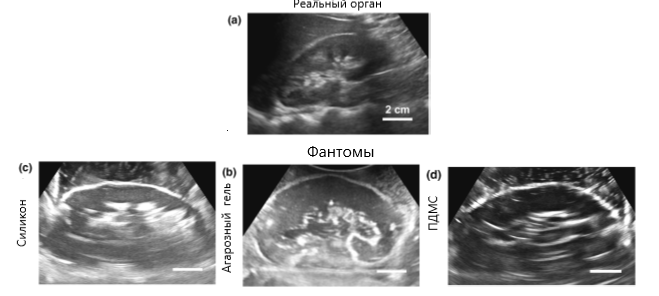
\includegraphics[width=0.9\textwidth]{Рисунки/УЗИ.png}
\caption{\centering Сравнение ультразвукового изображения фантомов из силикона, ПДМС и агарозного геля}.
\label{оболочка}
\end{center}
\end{figure}

В исследовании \cite{litlink53} используется другой тип гидрогелей - гелевый воск. Применяются две добавки к гелевому воску (углеводород с добавлением аполимера, модель FF1 003) - стеклянные сферы с номинальным диаметром от 0 до 63 мкм для увеличения акустического рассеяния и парафиновый воск для увеличения коэффициента затухания. Добавление парафина оказало сильное влияние на коэффициент затухания и слабое влияние на скорость звука и акустический импеданс. Коэффициент затухания быстро увеличивался с увеличением концентрации парафинового воска. Когда концентрация добавленного парафинового воска была увеличена до 8 \%, затухание увеличилось с 0,72 до 2,91 дБ/см на 3 МГц и на 10 МГц с 6,84 до 26,63 дБ/см. В том же диапазоне концентраций скорость звука существенно не изменилась. Скорость звука гелевого воска (1448,5 м/с) на 6,3 \% ниже, чем средняя скорость звука для мягких тканей (1540 м/с). Добавление стеклянных сфер для обеспечения обратного акустического рассеяния оказало заметное влияние на внешний вид ультразвука и не оказало существенного влияния на скорость звука и акустическое затухание.

Еще одним типом гидрогелей, используемых для изготовления фантома является ПВС. Фантомы на основе ПВС имеют низкую стоимость, неограниченный срок службы при хранении в воде, высокую структурную жесткость и требуют меньше ингредиентов по сравнению с более распространенными тканевыми заменителями на основе агарозы с добавками \cite{litlink54}. Однако довольно трудоемкая процедура подготовки этого материала является главным недостатком.

\subsection{ПДМС}

Фантомы ПДМС могут быть полезны для хирургического обучения, для моделирования таких процедур, как биопсия и введение иглы. Также ПДМС используется для имитации сосудов \cite{litlink54}. Но скорость звука и, следовательно, акустический импеданс ПДМС меньше по сравнению с тканью сосуда человека, что приводит к нехарактерным акустическим отражениям на стенке фантомного сосуда. Механические свойства ПДМС можно изменять, варьируя соотношение эластомера и отвердителя (например, изменив соотношение с 1:10 до 1: 5, скорость звука увеличится с 1076,5 до до 1119,5 м/с, а затухание снизится с 21,30 до 14,86 дБ/см на частоте 5 МГц) \cite{litlink55} или отверждая при различных температурах. 

\subsection{Силиконы}

Несмотря на распространенность агарозного геля, преимущественными материалами для фантома являются силиконовые материалы из-за их высокой прочности и простоты изготовления. Ниже будут рассмотрены свойства силиконов RTV615, Dragon Skin, Ecoflex 0010 и Ecoflex 0030. Эти силиконы обладают необходимыми механическими свойствами (способность сохранять свою форму, устойчивость к деградации), большим запасом прочности и уже испытывались в изготовлении фантомов.

Во всех силиконовых фантомах скорость звука составляет примерно 1000 м/с, и они имеют высокое затухание (обычно > 2 дБ/см). 

Фантомы из силиконов, в отличие от агара, стабильны в течение месяцев и даже лет и, в отличие от агара, нечувствительны к грубому обращению \cite{litlink56}. Как и агар, силикон не токсичен при приготовлении и применении. Время отверждения зависит марки силикона и от температуры, чем выше температура, тем меньше время отверждения. 

Из группы эластомеров, проанализированных в литературе, силиконовый каучук RTV615 является материалом с самым низким коэффициентом затухания (1,2-1,55 дБ/см*МГц), но его скорость звука равна 1080 м/с, что составляет 74\% от скорости звука в жировой ткани \cite{litlink46}. 

Dragon Skin –платиновый силикон с большой прочностью на разрыв, выдерживающий деформацию до 1000\%. \cite{litlink57}. Его главным преимуществом является то, что он имеет ту же скорость звука, что и мягкие ткани. Однако коэффициент затухания этого силикона немного выше по сравнению с тканями человека, что ограничивает глубину обзора при ультразвуковой визуализации.

В данный момент cиликоны Ecoflex представлены в четырех вариантах, различающихся степенью мягкости по Шору: 5, 00-30, 00-10 и 00-50 \cite{litlink58}. Ecoflex 0010 используется для имитации жировых тканей, Ecoflex 0030 для имитации кожи \cite{litlink59}. 

В исследовании \cite{litlink59} сравнивались механические свойства силиконов Ecoflex 0030, Ecoflex 00-10 и Dragon Skin. Результаты показали, что все три силиконовых состава имеют значения модуля сдвига, которые попадают в диапазон биологических тканей (от 11 до 105 кПа). 

По результатам проведенного анализа было определено 3 типа силикона, пригодных для изготовления мягких тканей и органов: Ecoflex 00-10, RTV615 и Dragon-Skin. 

Силикон Ecoflex 00-10 является наиболее распространенным непромышленным силиконом малой твердости. В отличие от Dragon-Skin, который используется в основном для многоразовых сердечных фантомов \cite{litlink60}, он протестирован в большим количеством добавок (графит, вазелиновое масло, Slacker, ПААГ), что позволит упростить процесс изготовления и варьирование его механических и акустических свойств.


\subsection {Добавки для силиконовых материалов}

Механические свойства силиконов изменяют, используя специальные добавки. Присутствие жидких добавок, увеличивает скорость звука, в то время как добавление твердых включений ее уменьшает \cite{litlink57}.

В \cite{litlink46} силикон RTV615 смешивался с силиконовым маслом 40\%, что снизило коэффициент затухания до интересующего диапазона значений, однако увеличения скорости звука не наблюдалось. Результаты исследования \cite{litlink46} показали, что путем добавления силиконового масла можно регулировать акустические свойства эластомера RTV615 до значений, приближающихся к значениям мягких биологических тканей, сохраняя их стабильность во времени. Считается, что при смешивании большой концентрации силиконового масла со смесью силиконового каучука (перед отверждением) материал приобретает самовосстанавливающиеся свойства \cite{litlink60}. Образцы самовосстанавливающихся силиконов имеют гелеобразный состав и должны быть заключены в более прочный силиконовый обволакивающий слой, защищающий их от окружающей среды и сохраняющий форму.  

Использование вазелина снижало значение затухания также, как добавление силиконового масла, и дало значительное увеличение скорости \cite{litlink46}. 
 
Добавление глицерина способствовало лучшему увеличению скорости, однако увеличивало коэффициент затухания \cite{litlink46}.

Благодаря использованию 75\% ПДМС с концевыми виниловыми группами в двухкомпонентной смеси силиконового эластомера SL-3358 \cite{litlink58}, скорость звука достигает значения 1290 м/с, а затухание 12,99 дБ/см при 5 МГц, которые соответствуют значениям для ткани груди человека. На рисунке 1.17 показаны ультразвуковые изображения фантома с различным содержанием ПДМС с концевыми виниловыми группами (разбавляющий агент) с частотой ультразвука 12 МГц.

Slacker (кремниевая жидкость) используется, чтобы улучшить механические свойства смеси и сделать ее более мягкой. Slacker позволяет изменять степень липкости затвердевшего силикона (степень пропорциональна количеству добавленного Slacker) и придает силикону свойство самоуплотнения, подобное тканям человека (способность снова закрываться после введения иглы). В \cite{litlink59} наилучшей добавкой к силикону Ecoflex 00-10 стал Slacker с 30\% концентрацией для фиброзной ткани (так как она является наиболее гипоэхогенной). 

ПААГ способствует повышению затухания пропорционально количеству добавленного геля при его массовой доле от 10 до 50\%. Образцы с добавкой ПААГ 20\% показали заметное увеличение эхогенности, поэтому они считаются хорошими кандидатами для имитации жировой ткани. Однако эта смесь нестабильна и через несколько недель теряет свои свойства, так как гидрофобный силикон отделяется от водосодержащего геля, а также из-за своей токсичности, в первую очередь во время приготовления, ПААГ нежелателен для изготовления фантомов.

Преимущественными в качестве добавок к силикону являются ПДМС с концевыми виниловыми связями в концентрациях от 50\% до 80\%, силиконовое масло PMX200 в концентрациях от 50\% до 87\%, а также Slacker в концентрациях от 10\% до 20\%, так как его максимальный процент смешиваемости составляет 20\% \cite{litlink60}. Данные добавки позволяют получить максимальное приближение скорости звука в материале и механические свойства к реальным биотканям.

\begin{figure}[H]
\begin{center}
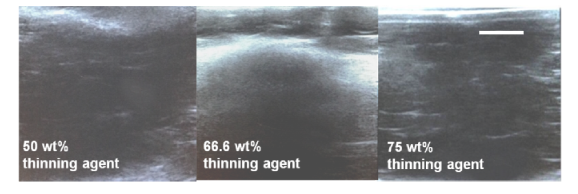
\includegraphics[width=0.8\textwidth]{Рисунки/ПДМС.png}
\caption{\centering Сравнение ультразвуковых изображений фантома с различным содержанием ПДМС}
\label{оболочка}
\end{center}
\end{figure}

\section{Выводы к главе 1}
В ходе проведенного медико-биологического обзора рассмотрены основные методы трекинга внутрисосудистых инструментов на изображениях с ультразвуковых визуализационных систем, проведен обзор существующих материалов для изготовления фантома мягких тканей, определены основные области применения роботизированных ультразвуковых систем, описана модель биологического объекта. По результатам обзора составлен лист постановки задачи, представленный в приложении A.








		%\chapter*{Введение}
%\addcontentsline{toc}{chapter}{Введение}

\newpage
\textbf{2 Проектирование БТС}
\refstepcounter{chapter}
\addcontentsline{toc}{chapter}{2 Проектно-конструкторская часть}
%\settocdepth{subsubsection}

\section{Разработка макета адаптера}
Позиционирование УЗ-датчика делится на два этапа: приблизительное размещение датчика в области исследования и более точная установка (выбор угла поворота и силы прижатия датчика). Для осуществления этих этапов необходимо разработать адаптер для крепления УЗ-датчика к конечному звену манипулятора, конструкция которого удовлетворяет следующим требованиям:

- возможность присоединения к конечному звену робота-манипулятора UR5e,

- обеспечение быстрого закрепления  и снятия ультразвукового датчика с помощью удобных для пользователя механизмов, 

- минимизация искажений измеренных сигналов на датчике силы, возникающих из-за сил тяжести, действующих на кабели устройства.

Исходя из геометрических параметров УЗ-датчика был спроектирован адаптер (рисунок 8а), состоящий из трех частей: основания (рисунок 8б), прижимной планки (рисунок 8в) и прижима провода (рисунок 8г).

Из-за криволинейной формы ручки датчика для надежности фиксации было выбрано винтовое соединение составных частей. 

Основание с помощью винтов прикручивается к конечному звену манипулятора, затем устанавливается УЗ-датчик и фиксируется прижимной планкой с помощью винтов. Для быстрого закрепления и снятия используются зажимные винты-барашки. Для обеспечения фиксации соединительного кабеля спроектирован прижим, который закрепляется на основании с помощью винтов со сферической головкой AS 1427H M4x16. 

\begin{figure}[H]
\begin{minipage}[h]{0.47\linewidth}
\center{\includegraphics[width=1\linewidth]{сборка.png}} a) \\
\end{minipage}
\hfill
\begin{minipage}[h]{0.47\linewidth}
\center{\includegraphics[width=1\linewidth]{основание.png}} \\б)
\end{minipage}
\vfill
\begin{minipage}[h]{0.47\linewidth}
\center{\includegraphics[width=1\linewidth]{планка.png}} в) \\
\end{minipage}
\hfill
\begin{minipage}[h]{0.47\linewidth}
\center{\includegraphics[width=1\linewidth]{прижим.png}} г) \\
\end{minipage}
\caption{3Д-модель макета адаптера для конечного звена манипулятора: a - адаптер в сборе; б - основание; в - планка прижимная; г - прижим провода}
\label{ris:experimentalcorrelationsignals}
\end{figure}

%Для данной конструкции выбрана однолистовая изогнутая пружина. Материал – АМг2М (сплав алюминия, легированного магнием и марганцем). Характеристики данной пружины следующие: 

%– давление (нагрузка на контакты) $P=0,4$ кг,

%– длина рабочей части пружины $L=30$ мм,

%– допускаемое напряжение на изгиб при переменной нагрузке $R_b=49$ кг/мм$^2$,

%– модуль упругости $E=7000$~кг/мм$^2$,

%– прогиб пружины $f=15$ мм. 


%Определим толщину пружины:\\
%\begin{equation}\label{tol}
%h=\frac{2\cdot L^2 \cdot R_b}{3 \cdot f \cdot E}.
%\end{equation}
%$h=0,28$ мм.

\section{Анализ технологичности конструкции макета адаптера}
Конструкция имеет простую компоновку и простое конструктивное решение, что не вызывает затруднений при сборке. В конструкции предусматриваются базовые детали, которые являются основой для расположения остальных составных частей узла. Масса всех деталей узла не превышает 0,5 кг. Можно легко производить замену деталей в процессе эксплуатации, что удешевляет ремонт. Конструкция сборочной единицы  обеспечивает возможность ее сборки из предварительно собранных составных частей.


Данное конструктивное решение позволяет выполнять все необходимые функции БТС и удовлетворяет всем требованиям для получения оптимального сигнала: обеспечивает точное позиционирование  спектрофотометрических датчиков на голове, не производит механическую нагрузку на исследуемую область, позволяет проводить измерения при движении пациента. Для улучшения конструкторской разработки можно увеличить количество каналов, что позволит проводить зондирование на разных расстояниях между источником и детектором.

\section{Прочностной расчет конструкции макета адаптера}
Для расчета конструкции на прочность в ПО Ansys смоделировано действие двух типов нагрузок (рисунок 2.7).
\begin{figure}[!h]
\begin{center}

\begin{minipage}[h]{0.45\linewidth}
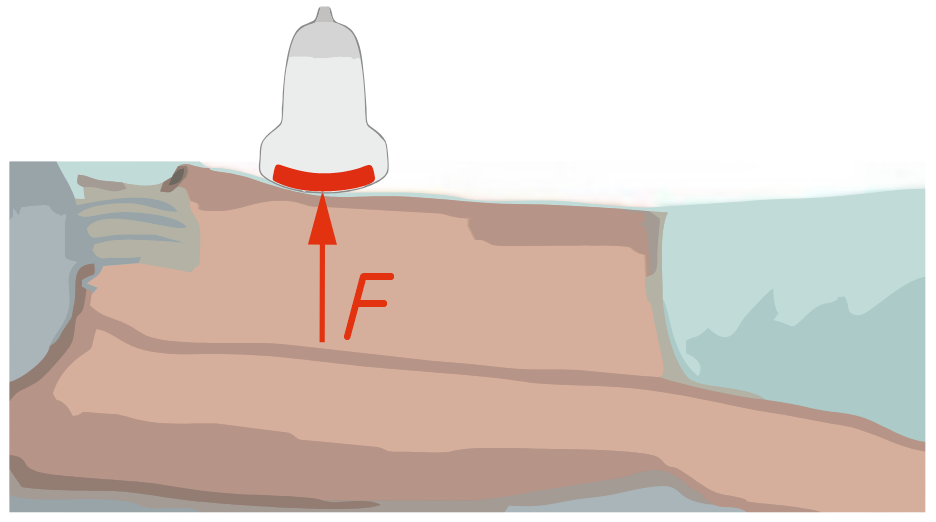
\includegraphics[width=\textwidth, keepaspectratio]{сила1}
\end{minipage}
%\hfill
\begin{minipage}[h]{0.45\linewidth}
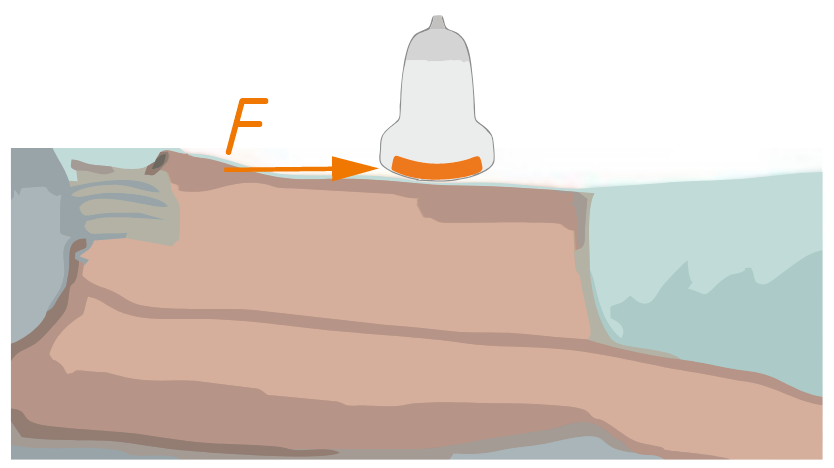
\includegraphics[width=\textwidth, keepaspectratio]{сила2}
\end{minipage}
\begin{minipage}[!h]{0.45\linewidth}
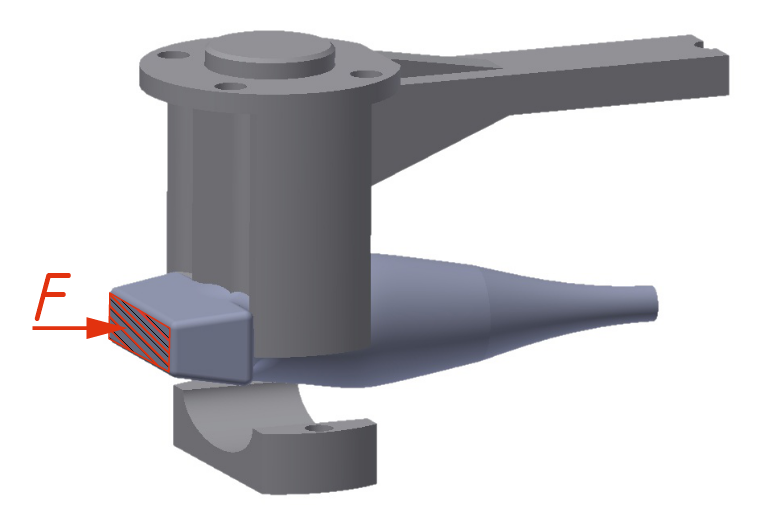
\includegraphics[width=\textwidth, keepaspectratio]{сила1адапт}
\end{minipage}
%\hfill
\begin{minipage}[h]{0.45\linewidth}
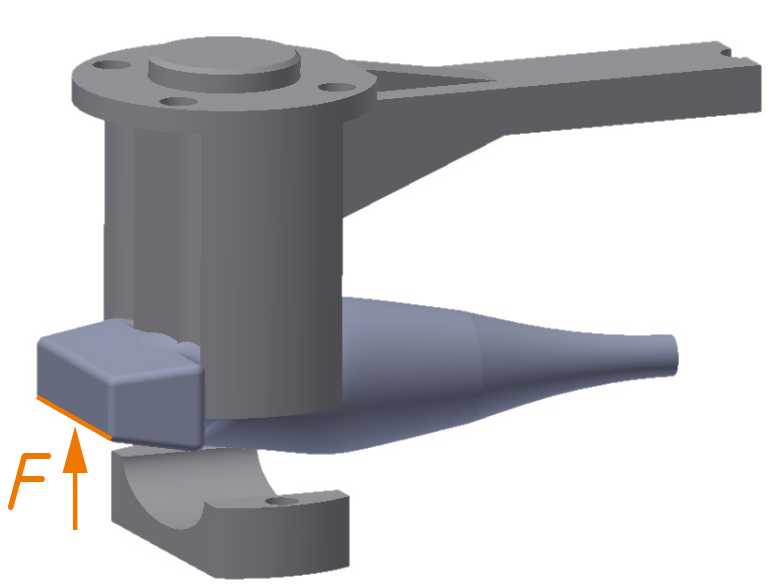
\includegraphics[width=\textwidth, keepaspectratio]{сила2адапт}
\end{minipage}
\caption{\centering \onehalfspacing {Типы нагрузок на УЗ-датчик}}
\label{risB}
\end{center}
\end{figure}

Первая нагрузка обусловлена действием силы реакции опоры со стороны тела пациента и распределена по выделенной поверхности датчика, вторая - неровностями поверхности тела, приложена к боковому ребру датчика (рисунок 2.7). Макет адаптера рассчитан диапазон действия сил от 10 до 100 Н. Для фиксации адаптера к манипулятору UR5e смоделирована фиксирующая заделка в месте закрепления адаптера. Для всех составных частей конструкции выбран материал ПВС, предел прочности при разрыв которого составляет 55 МПа. 

\section{Общий вид роботизированного комплекса}
На рисунке 9 представлен чертеж общего вида роботизированного комплекса, в котором предполагается использовать разрабатываемую БТС.

\begin{figure}[!h]
\begin{center}
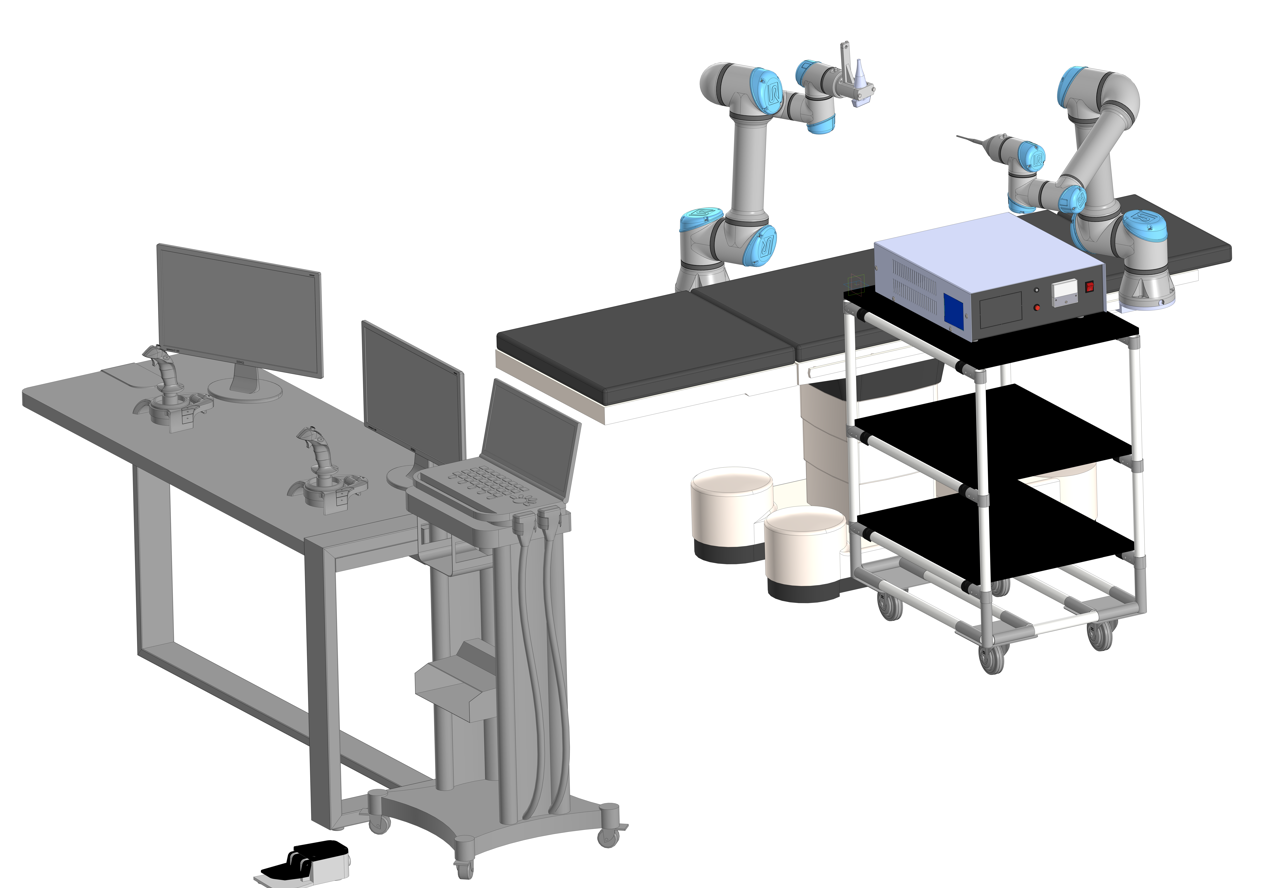
\includegraphics[width=\textwidth]{Рисунки/опер.png}
\caption{\centering \onehalfspacing {Чертеж общего вида роботизированного комплекса}}
\label{част}
\end{center}
\end{figure}

Операционный блок - специальное помещение хирургического отделения, предназначенное для выполнения операций и проведения мероприятий по их обеспечению. Операционный блок, оснащенный роботизированной системой, включает в себя операционный стол, по бокам которого расположены визуализирующий и хирургический манипуляторы, и УЗ-аппарат.Роботы-манипуляторы перемещаются вдоль операционного стола с помощью боковых рельсов, на которых закрепляются с помощью болтов. На конечном звене визуализирующего манипулятора закреплен УЗ-датчик с помощью разработанного адаптера. На хирургическом манипуляторе закреплен ультразвуковой узел.
\section{Система передачи УЗ-изображения на ПК}
В настоящее время существуют два способа передачи данных с ультразвукового аппарата: в режиме реального времени и путем сохранения, обработки и передачи данных для анализа. При использовании технологии сохранения/передачи данных исследование проводится дистанционно, полностью автономно, все УЗ-изображения сохраняются на сканере, а потом передаются для анализа. Такая технология не подходит для решения поставленных задач, так как врачу необходимо контролировать движение инструмента в режиме реального времени \cite{litlink1}.

В режиме реального времени происходит потоковая передача видеоизображения. Такая технология передачи данных более требовательна к пропускной способности канала связи. 

Наиболее часто используемая глубина пикселя ультразвукового изображения - 8 бит \cite{litlink2,litlink3}.

Допустимое разрешение в современных ультразвуковых исследованиях варьируется от 1024×1280 \cite{litlink4,litlink5} до 1366×768 \cite{litlink6}. 

Так как УЗ-аппарат Apogee 1100 имеет разрешение 1024×768, минимальное разрешение изображения должно быть 1024×768 пикселей. Также Apogee 1100 имеет выходы VGA и HDMI для извлечения видеопотока.

Для передачи ультразвуковых изображений в реальном времени требуется минимальная скорость передачи данных около 256 Кбит/с и минимальная частота кадров около 15 кадров в секунду. С таким техническими требованиями возможно проводить исследование в реальном времени и получать УЗ-изображения допустимого качества \cite{litlink7}.

В исследовании \cite{litlink3} устанавливается необходимая минимальная частота кадров для УЗИ - 25 кадров в секунду. Чем больше кадров в секунду, тем плавнее видеопоток. 

Аpogee 1100 имеет частоту кадров 2000 кадров/c. Так как частота обновления монитора намного меньше этого значения, допустимой видеограббера является его максимальная частота 60 fps. В исследовании \cite{litlink8} считается допустимой скорость передачи данных 800 Мбит/c (0,78 Гбит/c), а в работе \cite{litlink9} 0,1 Гбит/c. Исходя из этого, выберем оптимальной скорость передачи данных 1 Гбит/c.

Таким образом, технические требования к видеограбберу для захвата видеопотока с УЗИ-аппарата и передачи на ПК:

– захват VGA/HDMI сигнала,

– частота кадров 60 fps,

– поддержка разрешения 1024×768,

– глубина цвета – от 8 бит,

– скорость передачи данных – 1 Гбит/c.

Компактный внешний фрейм-граббер (рисунок 2), способный захватывать сигналы интерфейсов DVI и VGA с частотой обновления до 60 fps. Подключается к компьютеру через Ethernet порт, обеспечивая передачу данных со скоростью 1 Гбит/c. В устройстве имеется 3.5 мм аудиовход. 

\begin{figure}[H]
\begin{minipage}[h]{0.47\linewidth}
\center{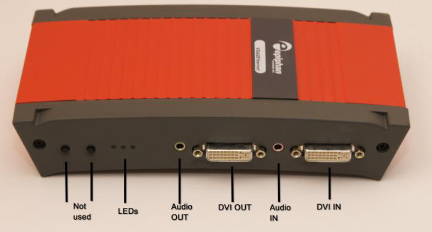
\includegraphics[width=1\linewidth]{граб1.png}} \\
\end{minipage}
\vfill
\begin{minipage}[h]{0.47\linewidth}
\center{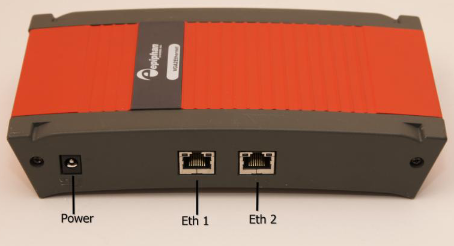
\includegraphics[width=1\linewidth]{граб11.png}} \\
\end{minipage}
\caption{Внешний вид устройства}
\label{ris:experimentalcorrelationsignals}
\end{figure}

Основные характеристики:

– поддержка интерфейсов DVI или VGA,

– частота кадров 60 fps,

– поддержка разрешений до 1920 х 1200,

– возможность работы по витой паре (Ethernet) с удаленно подключенным монитором либо проектором.

Стоимость устройства составляет 1600 долларов. 

На рисунке 3 показана схема подключения EPIPHAN VGA2Ethernet к системе.

\begin{figure}[!h]
\begin{center}
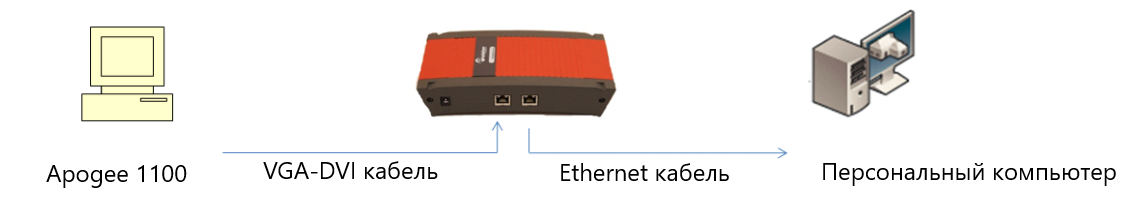
\includegraphics[width=\textwidth]{Схема граббер.png}
\caption{\centering \onehalfspacing {Схема подключения Apogee 1100 к ПК через EPIPHAN VGA2Ethernet}}
\label{част}
\end{center}
\end{figure}

Основные характеристики:

– захват изображения VGA,

– интерфейс USB 2.0,

– разрешение до 1920×1200,

– цветовое разрешение 16 бит/пиксель,

- выходной сигнал выводится c кадровой частотой от 3 до 28 Гц.

Частота обновления Epiphan VGA2USB при 1024×768 принимает значение 10 кадров в секунду. Это значение ниже допустимого порога, поэтому при использовании данного видеограббера необходимо дополнительно сжимать данные. Стоимость устройства составляет 500 долларов. 

На рисунке 4 показан внешний вид и разъемы Epiphan VGA2USB.

\begin{figure}[!h]
\begin{center}
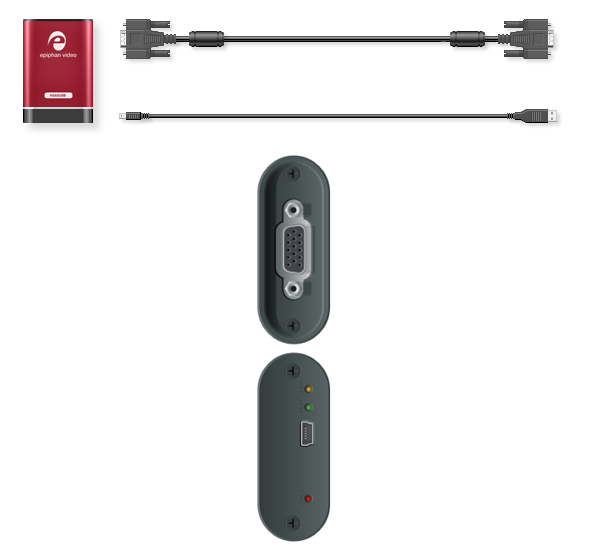
\includegraphics[width=0.6\textwidth]{граб2.png}
\caption{\centering \onehalfspacing {Внешний вид устройства}}
\label{част}
\end{center}
\end{figure}

Видеограббер позволяет выводить видеопоток с УЗ-аппарата через интерфейс VGA или DVI и передавать на ПК с помощью порта USB или Ethernet. Рассмотренные видеограбберы способны захватывать видеопоток в высоком качестве. Основным преимуществом  Epiphan VGA2USB и EPIPHAN VGA2Ethernet является то, что они поддерживают программную библиотеку для ультразвука (PLUS), которая представляет собой программный инструментарий с открытым исходным кодом для систем вмешательства под ультразвуковым контролем \cite{litlink5}. Устройства совместимы программами DirectShow и Video4Linux, что позволяет просматривать ультразвуковой видеопоток с помощью обычных видеоплееров.

\section{Решение кинематической задачи для манипулятора UR5e}

Прямая кинематическая задача заключается в расчете угла наклона конечного звена манипулятора, связанного с рабочим инструментом (УЗ-датчиком), при заданном наборе обобщенных координат остальных звеньев манипулятора.

Расположение и ориентация рабочего инструмента зависит от совместного действия вращения и/или переноса каждого сочленения цепи звеньев.  

Различают два базовых (элементарных) типа сочленений с одной степенью свободы: вращательный и поступательный. При наличии первого из них относительное расположение смежных звеньев определяется угловой переменной, при наличии второго — линейным смещением. В обоих случаях эти переменные называются обобщенными координатами:

\begin{equation}
q_{i}=\left\{\begin{array}{ll}
\theta_{i}, & \text { если звено } i \text { вращательное; } \\
d_{i}, & \text { если звено } i \text { поступательное. }
\end{array}\right.
\end{equation}

Известно, что положение и ориентация твердого тела в пространстве однозначно определяется шестью координатами: тремя линейными (декартовыми) и тремя угловыми (углами Эйлера). Использование метода Денавита-Хартенберга, позволяет сократить это число до четырех параметров, называемых параметрами Денавита-Хартенберга. Такое упрощение достигается с помощью стандартизированного алгоритма привязки систем координат к звеньям манипулятора.

Смысл введения локальных систем координат состоит в том, что поворот звена удобно выразить через поворот локальной системы координат относительно базовой, так как управление манипулятором фактически заключается в указании каждому звену обобщённых координат. Чтобы определить положение и ориентацию конечного звена, следует вычислить набор углов между сочленениями, которые приводят к соответствующей позиции рабочего инструмента. Как следствие, позиция рабочего инструмента манипулятора описывается не только в декартовых координатах, но также и в обобщённых.

Метод Денавита-Хартенберга состоит в формировании однородной матрицы преобразования, имеющей размерность 4х4 и описывающей положение системы координат каждого звена относительно системы координат предыдущего \cite{litlink10}. Это даёт возможность последовательно преобразовать координаты рабочего инструмента манипулятора из системы отсчёта, связанной с последним звеном, в базовую систему отсчёта.

Так как управление состоит в указании угла между двумя соседними звеньями – изменение этого угла приводит к изменению положения одной локальной системы координат относительно другой, что приводит к необходимости описывать каждую последующую локальную систему относительно предыдущей. Для описания изменения положения и ориентации одной локальной системы координат относительно предыдущей используются однородные матрицы преобразования.

Для описания геометрии робота-манипулятора UR5e (рисунок 5а) используется кинематическая схема, которая представляет собой графическое изображение последовательности звеньев манипулятора, соединенных между собой сочленениями (рисунок 5б).

\begin{figure}[H]
\begin{minipage}[h]{0.47\linewidth}
\center{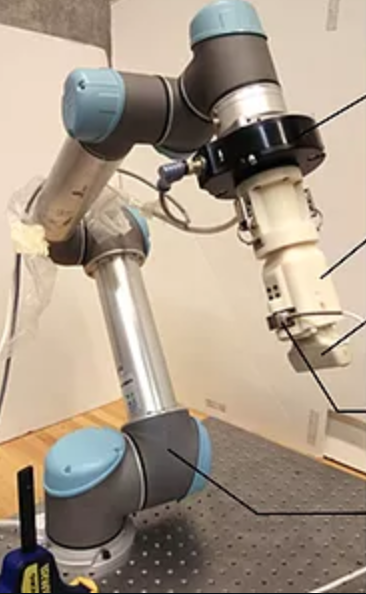
\includegraphics[width=0.5\linewidth]{сдатчиком.png}} \\a) 
\end{minipage}
\hfill
\begin{minipage}[h]{0.47\linewidth}
\center{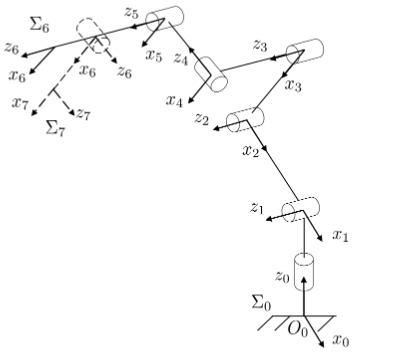
\includegraphics[width=0.9\linewidth]{кинематика1.png}} \\б)
\end{minipage}
\caption{Геометрия робота UR5e: а - робот-манипулятор с закрепленным датчиком, б - кинематическая схема (7-е звено принадлежит рабочему инструменту)}
\label{ris:experimentalcorrelationsignals}
\end{figure}

Представление Денавита-Хартенберга твёрдых звеньев зависит от четырёх геометрических параметров, соответствующих каждому звену. Эти четыре параметра полностью описывают любое вращательное или поступательное движение. Этот набор параметров достаточен для описания кинематической схемы каждого звена.

Кроме базовой системы координат для каждого звена на оси его сочленения определяется ортонормированная декартова система координат ($x_i$, $y_i$, $z_i$) , где $i=1..n$, а n равно числу степеней свободы
манипулятора (рисунок 6)\cite{litlink11}. 


\begin{figure}[!h]
\begin{center}
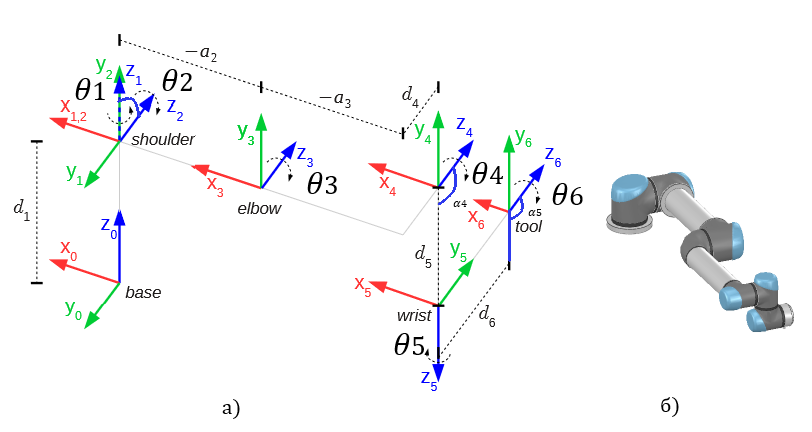
\includegraphics[width=1\textwidth]{кинематика2.png}
\caption{\centering \onehalfspacing {Определение параметров Денавита-Хартенберга: а - кинематическая схема с параметрами, б - визуализация на UR5e}}
\label{БТС}
\end{center}
\end{figure}

Поскольку вращательное сочленение имеет только одну степень свободы, каждая система координат ($x_i$, $y_i$, $z_i$) манипулятора соответствует $(i+1)$ сочленению и связана с $i$ звеном. Когда силовой привод возбуждает движение в $i$ сочленении, $i$ звено начинает двигаться относительно $(i-1)$ звена. Поскольку $i$  система координат связана с $i$  звеном, она движется вместе с ним. Таким образом, n-я система координат движется вместе с последним n-м звеном манипулятора.

$\boldsymbol{a}_{\boldsymbol{i}}$ - расстояние вдоль оси $x_{i}$ от $z_{i-1}$ до $z_{i}$;

$\boldsymbol{\alpha}_{\boldsymbol{i}}$ - угол вокруг оси $x_{i}$ от $z_{i-1}$ до $z_{i}$;

$\boldsymbol{d}_{\boldsymbol{i}}$ -  расстояние вдоль оси $z_{i-1}$ от $x_{i-1}$ до $x_{i}$;

$\boldsymbol{\theta}_{\boldsymbol{i}}$ - угол вокруг оси $z_{i-1}$ от $x_{i-1}$ до $x_{i}$.

Из четырёх параметров ($\boldsymbol{\theta}_{\boldsymbol{i}}, \boldsymbol{d}_{\boldsymbol{i}}, \boldsymbol{a}_{\boldsymbol{i}}, \boldsymbol{\alpha}_{\boldsymbol{i}}$) два параметра $\boldsymbol{\alpha}_{\boldsymbol{i}}$ и $\boldsymbol{a}_{\boldsymbol{i}}$  всегда  постоянны и  определяются  конструкцией  робота.  Один  из  двух  других параметров ($\boldsymbol{\theta}_{\boldsymbol{i}}$ либо $\boldsymbol{d}_{\boldsymbol{i}}$)  является  переменным.  Для вращательного  сочленения  величина $\boldsymbol{\theta}_{\boldsymbol{i}}$ характеризует  угол  относительного  поворота  звеньев  $i-1$  и  $i$,  а  линейная  величина $\boldsymbol{d}_{\boldsymbol{i}}$ постоянна. 

При решении прямой задачи рассматриваются две системы координат: исходная (базовая), связанная с «землей»,
$o_{0} x_{0} y_{0} z_{0}$ и итоговая $o_{n} x_{n} y_{n} z_{n}$, связанная с рабочим инструментом.

Рассмотрим подробнее два набора координат $k_{0}$ и $k_{n}$ одной и той же точки в пространстве, выраженные относительно систем $o_{0} x_{0} y_{0} z_{0}$ и $o_{n} x_{n} y_{n} z_{n}$, соответственно:

\begin{equation}
k^{0}=T_{n}^{0} k^{n},
\end{equation}

где $T_{n}^{0}$ - преобразование, несущее информацию о линейном смещении и пространственной ориентации одной системы относительно другой.

Когда системы координат сформированы для всех звеньев, можно построить однородные матрицы преобразования, связывающие i-ю и i-1-ю системы координат \cite{litlink10}:

\begin{equation}
A_{i}=\left[\begin{array}{cccc}
\operatorname{Cos} \theta_{i} & -\operatorname{Sin} \theta_{i} \operatorname{Cos} \alpha_{i} & \operatorname{Sin} \theta_{i} \operatorname{Sin} \alpha_{i} & \alpha_{i} \operatorname{Cos} \theta_{i} \\
\operatorname{Sin} \theta_{i} & \operatorname{Cos} \theta_{i} \operatorname{Cos} \alpha_{i} & -\operatorname{Cos} \theta_{i} \operatorname{Sin} \alpha_{i} & \alpha_{i} \operatorname{Sin} \theta_{i} \\
0 & \operatorname{Sin} \alpha_{i} & \operatorname{Cos} \alpha_{i} & d_{i} \\
0 & 0 & 0 & 1
\end{array}\right]
\end{equation}

Для того, чтобы получить координаты последней, шестой локальной системы координат относительно базовой необходимо провести последовательно цепочку преобразований локальных систем. Таким образом, кинематическое положение рабочего инструмента может быть получено последовательным преобразованием координат точки $R_{i} (r_{xi}, r_{yi}, r_{zi})$ из одной системы координат $i$ в другую систему координат $i-1$ следующим образом:

\begin{equation}
\begin{aligned}
&R_0=A_1*R_1, \\
&R_1=A_2*R_2, \\
&R_2=A_3*R_3, \\
&R_3=A_4*R_4, \\
&R_4=A_5*R_5, \\
&R_5=A_6*R_6.
\end{aligned}
\end{equation}

Получим:

\begin{equation}
R_0=A_1*A_2*A_3*A_4*A_5*A_6*R_6,
\end{equation}

где $A_1*A_2*A_3*A_4*A_5*A_6 = T_{6}$.

Произведение матриц преобразования также даёт матрицу преобразования, поэтому матрица $T_6$ в итоге является матрицей А и имеет такую же структуру. Матрицу $T$ называют однородной матрицей композиции преобразования. В матрице $T$ вектор $p$ является координатой центра рабочего инструмента – вектор положения, а единичные векторы, определяющие ориентацию рабочего инструмента в базовой системе называются соответственно векторами подхода – $a$, ориентации – $o$, и нормали – $n$, все они образуют правостороннюю систему координат (рисунок 7) \cite{litlink12}.

\begin{figure}[!h]
\begin{center}
\begin{minipage}[h]{0.4\linewidth}
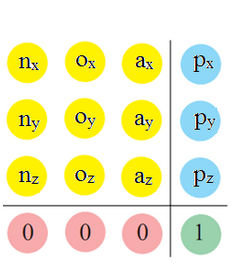
\includegraphics[width=\textwidth, keepaspectratio]{матрица.png}
\end{minipage}
%\hfill
\begin{minipage}[h]{0.4\linewidth}
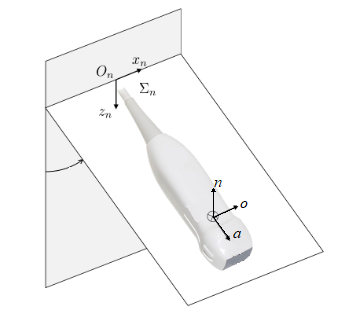
\includegraphics[width=\textwidth, keepaspectratio]{оси.png}
\end{minipage}
\caption{\centering \onehalfspacing {Структура матрицы $T_6$ и единичные векторы, определяющие ориентацию рабочего инструмента, желтым выделена матрица вращения, а синим - координаты центра рабочего инструмента}}
\label{risB}
\end{center}
\end{figure}

Так как каждый из этих векторов может быть получен в результате векторного произведения двух других, то для однозначного неизбыточного определения ориентации в пространстве достаточно выбрать любые два вектора из этой тройки.

В таблице 3.1 указаны параметры Денавита-Хартенберга для используемого робота UR5e \cite{litlink13}. Зная 6 матриц для каждого звена и, рассчитав с их помощью результирующую матрицу $T_{6}$, можно определить положение рабочего инструмента в пространстве.

\begin{table}[h]
\captionsetup[table]{singlelinecheck=false,justification=raggedleft}
\ttabbox
{\caption {\onehalfspacing Параметры Денавита-Хартенберга для робота UR5e}}
{\begin{tabular}{| >{\centering\arraybackslash}m{1.1in} | >{\centering\arraybackslash}m{1.1in} | >{\centering\arraybackslash}m{1.2in} | >{\centering\arraybackslash}m{1.2in}| >{\centering\arraybackslash}m{1.1in}|}
\hline 
Номер звена & $\boldsymbol{\theta_\boldsymbol{i}}$, рад & $\boldsymbol{a}_{\boldsymbol{i}}$, м & $\boldsymbol{d}_{\boldsymbol{i}}$, м & $\boldsymbol{\alpha}_{\boldsymbol{i}}$, рад \\ 
\hline
1 & $\boldsymbol{\theta_\boldsymbol{1}}$ & 0 & 0,1625 & $\pi/2$ \\
\hline
2 & $\boldsymbol{\theta_\boldsymbol{2}}$ & -0,4250 & 0 & 0 \\
\hline
3 & $\boldsymbol{\theta_\boldsymbol{3}}$ & -0,3922 & 0 & 0 \\
\hline
4 & $\boldsymbol{\theta_\boldsymbol{4}}$ & 0 & 0,1333 & $\pi/2$ \\
\hline
5 & $\boldsymbol{\theta_\boldsymbol{5}}$ & 0 & 0,0997 & $-\pi/2$ \\
\hline
6 & $\boldsymbol{\theta_\boldsymbol{6}}$ & 0 & 0,0996 & 0 \\
\hline
\end{tabular}}
\end{table}

Обратная задача кинематики заключается в расчете обобщенных координат при заданных линейных и угловых координатах рабочего инструмента манипулятора. Эта задача является более сложной, чем прямая, поскольку имеет 8 решений для манипулятора с 6 степенями свободны, т.е. одному и тому же положению рабочего инструмента в пространстве могут соответствовать разные конфигурации робота. 

Исходными данными являются параметры Денавита-Хартенберга и матрица $T_{6}$. Матрица вращения находится из $T_{6}$ (выделена желтым на рисунке 7) и имеет вид:

\begin{equation}
R_{n}^{0}(q)=\left[\begin{array}{lll}
r_{11}(q) & r_{12}(q) & r_{13}(q) \\
r_{21}(q) & r_{22}(q) & r_{23}(q) \\
r_{31}(q) & r_{32}(q) & r_{33}(q) 
\end{array}\right].
\end{equation}

Используя эти данные, находим $\theta$ для звена 1,5,6 \cite{litlink14}:

\begin{equation}
\theta_{1}=& \operatorname{arctg}\left(p_{y}-d_{6} r_{23}, p_{x}-d_{6} r_{13}\right)+\frac{\pi}{2} \\
& \pm \arccos \left(\frac{d_{4}}{\sqrt{\left(p_{y}-d_{6} r_{23}\right)^{2}+\left(p_{x}-d_{6} r_{13}\right)^{2}}}\right),
\end{equation}

\begin{equation}
\theta_{5}=\pm \arccos \left(\frac{p_{x}\operatorname{sin} \theta_{1}-p_{y}\operatorname{cos} \theta_{1}-d_{4}}{d_{6}}\right),
\end{equation}

\begin{equation}
\theta_{6}=\operatorname{arctg}\left(\frac{\operatorname{cos} \theta_{1} r_{22}-\operatorname{sin} \theta_{1} r_{12}}{\operatorname{sin} \theta_{5}}, \frac{\operatorname{sin} \theta_{1} r_{11}-\operatorname{cos}\theta_{1} r_{21}}{\operatorname{sin} \theta_{5}}\right).
\end{equation}
\\

Для нахождения $\theta_\boldsymbol{2}$, $\theta_\boldsymbol{3}$ и $\theta_\boldsymbol{4}$ рассчитаем $A_{3}$, $B_{3}$, $A_{4}$, $B_{4}$, $C_{4}$ и $D_{4}$:

\begin{equation}
\begin{aligned}
A_{3}=d_{5} \operatorname{sin} \theta_{6}\left(\operatorname{cos} \theta_{1} r_{11}+\operatorname{sin} \theta_{1} r_{21}\right)+d_{5} \operatorname{cos} \theta_{6}\left(\operatorname{cos} \theta_{1} r_{12}+\operatorname{sin} \theta_{1} r_{22}\right)\\-d_{6}\left(\operatorname{cos} \theta_{1} r_{13}+\operatorname{sin} \theta_{1} r_{23}\right)+p_{x} \operatorname{cos} \theta_{1}+p_{y} \operatorname{sin} \theta_{1},
\end{aligned}
\end{equation}

\begin{equation}
B_{3}=d_{5}\left(\operatorname{sin} \theta_{6} r_{31}+\operatorname{cos} \theta_{6} r_{32}\right)-d_{6} r_{33}+p_{z}-d_{1}.
\end{equation}

\begin{equation}
\begin{aligned}
&A_{4}=\operatorname{cos} \theta_{1} r_{11}+\operatorname{sin} \theta_{1} r_{21}, \\
&B_{4}=\operatorname{cos} \theta_{1} r_{12}+\operatorname{sin} \theta_{1} r_{22}, \\
&C_{4}=\operatorname{cos} \theta_{1} r_{13}+\operatorname{sin} \theta_{1} r_{23}, \\
&D_{4}=\operatorname{cos} \theta_{6} r_{31}-\operatorname{sin} \theta_{6} r_{32}.
\end{aligned}
\end{equation}

Тогда:

\begin{equation}
\theta_{3}=\pm \arccos \left(\frac{A_{3}^{2}+B_{3}^{2}-a_{2}^{2}-a_{3}^{2}}{2 a_{2} a_{3}}\right),
\end{equation}

\begin{equation}
\theta_{2}=\arcsin \left(\frac{-\operatorname{sin} \theta_{3} a_{3}}{\sqrt{A_{3}^{2}+B_{3}^{2}}}\right)+\operatorname{arctg}\left(B_{3}, A_{3}\right),
\end{equation}

\begin{equation}
\begin{aligned}
\operatorname{cos} \theta_{4}=\operatorname{cos}\left(\theta_{3}+\theta_{2}\right)\left(\operatorname{cos}\theta_{5} \operatorname{cos}\theta_{6} A_{4}-\operatorname{cos}\theta_{5} \operatorname{sin}\theta_{6} B_{4}-\operatorname{sin}\theta_{5} C_{4}\right)\\ + \operatorname{sin}\left(\theta_{3}+\theta_{2}\right)\left(\operatorname{cos} \theta_{5} D_{4}-\operatorname{sin} \theta_{5} r_{33}\right),
\end{aligned}
\end{equation}

\begin{equation}
\begin{aligned}
\operatorname{sin}\theta_{4}=\operatorname{sin}\left(\theta_{3}+\theta_{2}\right)\left(-\operatorname{cos} \theta_{5} \operatorname{cos} \theta_{6} A_{4}+\operatorname{cos} \theta_{5} \operatorname{sin} \theta_{6}B_{4}+\operatorname{sin} \theta_{5}C_{4}\right)\\+\operatorname{cos}{\theta_{3}+\theta_{2}}\left(\operatorname{cos} \theta_{5} D_{4}-\operatorname{sin} \theta_{5} r_{33}\right),
\end{aligned}
\end{equation}


\begin{equation}
{\theta_{4}=\operatorname{arctg}\left(\operatorname{sin} \theta_{4}, \operatorname{cos} \theta_{4}\right)}.
\end{equation}



\section{Выводы к главе 2}
В ходе проектирования биотехнической системы были сформулированы техническое задание и требования к БТС, в соответствии с требованиями разработана БТС, структурная и функциональная схемы, представленные в приложении А (рисунок А.2 и рисунок А.3). В части аппаратной реализации описан алгоритм работы все составных блоков аппаратной части, сформирована элементная база с учетом выполняемых системой задач. 

		\newpage
\textbf{3 Исследование и анализ вызванной динамики сигналов}
\refstepcounter{chapter}


\addcontentsline{toc}{chapter}{3 Научно-исследовательская часть}

\section{Биотехническая система для роботизированной
ультразвуковой визуализации}
\begin{figure}[!h]
\begin{center}
\includegraphics[width=\textwidth]{БТС.pdf}
\caption{\centering \onehalfspacing {Структурная схема БТС объективного контроля слухового восприятия спектрофотометрическим методом}}
\label{БТС}
\end{center}
\end{figure}

Для разработки БТС для неинвазивного измерения параметров гемодинамики височных долей коры головного мозга с помощью спектрофотометрического метода при одновременной подаче звуковых сигналов необходимо выполнить следующие задачи:

– определение необходимых технических требований к конструкции БТС,

– моделирование всех блоков системы,

– выбор комплектующих всех составных частей каждого блока,

– разработка конструкторской документации

– анализ технологичности конструкции изделия.

\subsection{Требования к конструкции БТС}
Основными задачами данной разработки является повышение точности позиционирования оптических датчиков при билатеральных измерениях (слева и справа) за счёт проектируемой конструкции и объединение устройства подачи звукового сигнала со спектрофотометрическими датчиками. Исходя из этого, сформулированы следующие требования к конструкции БТС:

– конструкция должна обеспечивать надежную фиксацию датчиков на голове пациента, их точное позиционирование,

– изделие должно быть устойчиво к двигательным артефактам,

– изделие должно обеспечивать возможность регулирования параметров таких параметров, как частота и амплитуда звукового сигнала, включение/выключение нужных каналов,

– фиксация датчиков на голове пациента не должна приводить к повреждающему механическому воздействию,

– изделие должно быть устойчиво по отношению к любым методам стерилизации или дезинфекции,

– масса изделия до 1 кг (без беспроводного блока передачи данных),

– обеспечение шумоподавления.

Технические требования:

– входное напряжение 7,5 В,

– непрерывный режим работы источников,

– 4 канала,

– мощность не более 5 мВт.


\subsection{Описание конструкции блоков}
Конструкция состоит из 5 блоков: блока подачи аудиосигнала (наушники), датчиков fNIRS, блока питания, блока обработки сигнала, Bluetooth-модуля. Конструкторская разработка проводилась для первых 2-х блоков.

В качестве блока подачи аудиосигнала могут выступать аудиометрические наушники с хорошей шумоизоляцией. В соответствии с вышеизложенными задачами, конструктивно он должен состоять из следующих частей: дуги наушников, подвижной части корпуса (вращательное движение), накладок и составного динамика. Для обеспечения удобной фиксации на голове пациента в дугу наушников встроены рейки, позволяющие регулировать положение накладок по высоте. Рейки закреплены с помощью реечного фиксатора. Нижний корпус вращается с помощью узла вращения, что обеспечивает плотное прилегание накладок к ушам. На рисунке \ref{ushi} показано взаимное расположение элементов данного блока.

\begin{figure}[!h]
\begin{center}
\includegraphics[width=0.5\textwidth]{12.pdf}
\caption{\centering Элементы блока подачи аудиосигнала}
\label{ushi}
\end{center}
\end{figure}

Два симметрично расположенных датчика должны покрывать височную долю коры головного мозга, длина которой около 70 мм, а ширина 30 мм \cite{litlink11}. Слуховые центры расположены в верхней височной извилине, которая находится примерно на 2 см выше уха. Конструкция должна обеспечить точное проецирование поверхности датчика на слуховую кору. Геометрическое расположение четырех световых излучателей и детектора на модуле показано на рисунке \ref{vis}. Детектор расположен в центре устройства, четыре светодиода расположены в противоположных углах на равных расстояниях 38 мм от детектора, которые закреплены с помощью стальных шарнирных штифтов диаметром 2 мм. Для оптимального качества сигнала важно, чтобы детектор света и излучатели находились как можно ближе к коже головы, но в то же время были перпендикулярны поверхности для обеспечения максимальной чувствительности и проникновения света. Чтобы  минимизировать влияние на сигнал из-за перемещения головы, конструкция светодиодов должна включать в себя пружины. Светодиоды не жестко соединены с корпусом датчика, а встроены в подвижные держатели и могут вращаться вокруг оси. Пружина прижимает светодиод к поверхности головы, тем самым обеспечивая предотвращая потерю контакта во время движения. Поворотное соединение удерживают светодиод перпендикулярно к поверхности, обеспечивая при этом небольшие отклонения для удобства. Подпружиненные светодиодные держатели построены с использованием 20 длинных акриловых стеклянных трубок с наружным диаметром 6 мм, длинных алюминиевых трубок с наружным диаметром 7 мм и толщиной стенки 0,5 мм и 18 мм-длинных металлических пружин с диаметром 4 мм. Многоволновой светодиод припаян к 3-проводному ленточному кабелю, который затем проходит через стеклянную трубку и металлическую пружину. Также светодиод заключен в толстую непрозрачную трубку из резины для предотвращения рассеянного света и амортизации. Для уменьшения влияния рассеянного света и для амортизирующих целей детектор заключен в непрозрачную резиновую трубку. Кроме того, корпус датчика fNIRS может быть окрашен непрозрачной черной краской с внутренней стороны для минимизации световых эффектов на датчик с направлений, отличных от перпендикулярных к чувствительной поверхности. 

Конструктивное решение закрепления датчиков на корпусе наушников – листовая пружина, закрепленная на винтах в нижнем корпусе и на корпусе датчика, что позволяет за счёт изгиба держать нагрузку и давить вперёд в сторону головы (рис. \ref{пруж}). Крепление корпуса датчика к стойке осуществляется за счет стальных шарнирных штифтов диаметром 4 мм (рис. \ref{соед}).

Проанализировав из каких составных элементов состоит каждый блок, составим список покупных изделий:\\
Покупные элементы блока:

– светодиоды (4 шт.),

– детектор,

– 8 винтов А.M3-6gx5,

– акустический кабель AW208.

\begin{figure}[!h]
\begin{center}
\includegraphics[width=0.5\textwidth]{соед.png}
\caption{\centering Закрепление корпуса датчика к листовой стойке}
\label{соед}
\end{center}
\end{figure}
В качестве излучаещего устройства можно использовать только лазерные диоды (ЛД) и светоизлучающие диоды (светодиоды) \cite{litlink15}. ЛД имеют высокую интенсивность излучения, могут быть использованы для получения высококачественного сигнала fNIRS. С другой стороны, их недостатки (перегрев, более высокие требования к безопасности, высокая стоимость и ограниченная длина волны) не позволяют использовать их в портативном устройстве. Поскольку светодиоды малы, сравнительно дешевы, имеют большой разброс по длинам волн, а проблемы нагрева менее критичны, они являются более подходящими для данной конструкции. Светодиоды позволяют проводить исследование одновременно с двух длин волн, что необходимо для расчета относительных показателей при непрерывном режиме. В исследовании \cite{litlink23} пришли к выводу, что использование длин волн 830 нм и 690-750 нм является оптимальным решением. Основываясь на анализе трехслойной модели, авторы работы \cite{litlink24} определили, что предпочтительные длины волн - 887 и 704 нм. Усредним эти результаты и выберем светодиод с длинам волн 760 и 850 нм. 

В роли детектора был выбран кремниевый фотодиод для детектирования света в системе fNIRS. Его преимуществами являются: маленький размер, высокий динамический диапазон и скорость работы. Еще одно преимущество заключается в том, что он может соприкасаться непосредственно с поверхностью кожи, что является наиболее эффективным методом. Из-за фиксированной модуляции оптического сигнала необходима полоса пропускания в несколько кГц. С учетом максимальной чувствительности и минимального уровня шума был выбран детектор OPT101. Он представляет собой монолитный фотодиод с одним источником питания и интегрированным трансимпедансным усилителем.

\begin{figure}[!h]
\begin{center}
\includegraphics[width=0.5\textwidth]{височная.pdf}
\caption{\centering \onehalfspacing {Приблизительное расположение источников и детектора на датчике в проекции на височную долю: красные точки - источники, черная - детектор, синие - точки наивысшей чувствительности к функциональной активности коры головного мозга}}
\label{vis}
\end{center}
\end{figure}

\section{Исследование акустических и механических параметров смеси ПВС-ПДМС}
Данное исследование было проведено для изучения возможностей метода К-БИК спектрофотометрии в оценке и контроле слухового восприятия. Целью эксперимента являлось измерение динамических изменений в концентрациях гемоглобина при стимуляции слуховой коры относительного исходных значений (среднее значение в покое) и разработка алгоритма обработки. Так как абсолютные значения параметров для этого не требуются, был выбран непрерывный режим, позволяющий отследить относительные показатели. 

\subsection{Описание и методика эксперимента}
Эксперимент проводился при помощи спектофотометрического прибора – тканевого оксиметра «OxiplexTS» и калибровочных блоков.

OxiplexTS – устройство, позволяющее измерять концентрацию оксигенированного и дезоксигенированного гемоглобина в тканях. Устройство работает, излучая ближний инфракрасный свет (NIR) в ткани на известных расстояниях от детектора. Используется свет двух различных длин волн (692 и 834 нм), который модулируется на радиочастотной частоте 110 МГц \cite{litlink26}. Собранный свет измеряется и обрабатывается, а также определяются коэффициенты поглощения и рассеяния среды. После определения поглощения и рассеяния применяется предположение о том, что гемоглобин является единственным значимым поглотителем, и вычисляются концентрации оксигенированного и деоксигенированного гемоглобина. OxiplexTS использует теорию миграции фотонов через сильно рассеивающие среды. Это позволяет проводить абсолютные измерения поглощения и рассеяния в высоко рассеивающей среде, такой как человеческая ткань.

Устройство измеряет следующие параметры в единицах АЦП (AC - амплитуда модуляции, DC – средний уровень интенсивности, Phase – фазовый сдвиг сигнала в градусах). Чтобы получить затухающие интенсивности с разных расстояний, надо AC или DC умножить на соответствующий калибровочный коэффициент, а к фазе – прибавить соответствующий калибровочный коэффициент. В данном эксперименте важны только относительные показатели поглощения и концентраций хромофоров, поэтому используется непрерывный режим модуляции. Частота дискретизации была выбрана 5 Гц (измерения проводились каждые 0,2 секунды). Так как измерения ведутся в непрерывном режиме, который чаще всего используется для картирования и также используется в конструкторской разработке, то из измеренных данных использовались значения DC (1-8) и рассчитывались сначала относительные изменения коэффициента поглощения для двух длин волн, по которым с учётом процентного содержания воды определяются относительные изменения концентраций окси-, дезокси- и общего гемоглобина. На первое измеренное значение DC(t0) нормировались все остальные измерения. На рисунке показано расположение источников (диодов) разных длин волн и расстояний. 

Протокол измерений был следующим: испытуемый сидит на стуле. Датчик канала А (Oxiplex) расположен с левой стороны над ухом; датчик канала В – с правой стороны над ухом. Точность позиционирования линейного 4-х-дистантного датчика в области проекции слуховой коры на поверхности головы никак не контролировалась. Оба датчика (каналов А и В) калибровались на церебральном блоке с указанными коэффициентами поглощения и транспортного рассеяния для обеих длин волн зондирующего излучения. На голове испытуемого были надеты внешние наушники, звуковой сигнал подавался в оба уха одновременно. Сигнал записывался десять минут, в течение которых чередовались измерения в покое (3 минуты) и измерения во время стимула (2 минуты). В качестве стимуляции слуховой коры был выбран текст аудиокниги. Повторная стимуляция была проведена для того, чтобы исключить сигналы, не связаные с вызванной активностью головного мозга.

\begin{figure}[!h]
\begin{center}
\includegraphics[width=0.5\textwidth]{датчик.png}
\caption{\centering Схема многодистантного оптоволоконного датчика}
\label{дат}
\end{center}
\end{figure}

\subsection{Анализ полученных данных}

\section{Исследование зависимости качества ультразвукового изображения от силы и угла прижатия УЗ-датчика}
\subsection{Показатели качества изображений с ультразвуковых визуализационных систем}
\subsection{Алгоритм работы программы для роботизированной УЗ-визуализации}
\subsection{Описание и методика эксперимента}
\subsection{Составление соответствующих выводов о влиянии механических параметров (силы и угла наклона) на полученное УЗ-изображение}

\section{Выводы к главе 3}
Все зарегистрированные сигналы были импортированы в MATLAB для дальнейшей обработки. На рисунке \ref{45} изображена схема реакции организма на внешний стимул. Можно заметить, что гемодинамические изменения происходят через 2–5 с после начала стимуляции. Этот факт нужно учитывать, анализируя полученные данные.

Расчет изменений концентраций окси, дезокси- и общего гемоглобина проводился в среде MATLAB по следующему алгоритму:

– умножаем значения DC на калибровочный коэффициент,
    
– с помощью модифицированного закона Бугера-Ламберта-Бера (\ref{blb}) находим относительные коэффициенты поглощения ($\Delta \mu_a$),

– решаем линейную систему уравнений с двумя неизвестными (\ref{konz}),

– находим $\Delta C_{HbO_2}$ и $\Delta C_{HHb}$,

– вычисляем $\Delta C_{THb}$ по формуле \ref{ob}.

\begin{figure}[!h]
\begin{center}
\includegraphics[width=\textwidth]{схемочка.pdf}
\caption{\centering Схема реакции организма на стимул}
\label{45}
\end{center}
\end{figure}

Так как биоткань является неоднородной средой с большим количеством поглощающих веществ, ослабление интенсивности света происходит согласно модифицированному закону Бугера-Ламберта-Бера:
\begin{equation}\label{blb}
I=I_0\cdot e^{-\mu_a \cdot r \cdot DPF},
\end{equation}

где $I$ и $I_0$ -- 
это интенсивности выходящего и входящего из ткани излучения соответственно;

$\mu_a$ - коэффициент поглощения среды (1/см);

$r$ - толщина слоя вещества, через которое проходит свет (см);

$DPF$ - параметр дифференциального пробега фотона, учитывающий увеличение пути миграции фотонов за счет рассеяния.

$DPF$ зависит от пола, возраста и длины волны. Для этого эксперимента выбраны усредненные значения для $\lambda= 692$ нм $DPF = 6.51$, а для $\lambda= 834$ нм $DPF = 5.86$.
Коррекция закона с помощью DPF не так важна, поскольку для данных задач не нужна количественная оценка параметров, а достаточно определить присутствует ли активация и в каких именно областях она происходит.

Подставляя значения измеренных интенсивностей в моменты времени $t_i$ и $t_{i+1}$, находим $\Delta \mu_a$:
\begin{equation}\label{blb}
\begin{cases}
   {I_i=I_0 \cdot e^{-\mu_{a,i}\cdot r \cdot DPF}}\\
   {I_{i+1}=I_0\cdot e^{-\mu_{a,{i+1}}\cdot r \cdot DPF}}
 \end{cases}
 \Rightarrow
 \begin{cases}
   {ln{\frac{I_0}{I_i}}=\mu_{a,i} \cdot r \cdot DPF}\\
   {ln{\frac{I_0}{I_{i+1}}}=\mu_{a,{i+1}} \cdot r \cdot DPF},
 \end{cases}
\end{equation}
\vspace{-5mm}

где $I_i$ и $I_{i+1}$ - интенсивности в моменты времени $t_i$ и $t_{i+1}$ соответственно (шаг по времени равен 0.2 секунды); 

$\mu_{a,i}$ и $\mu_{a,{i+1}}$ - коэффициенты поглощения ткани в моменты времени $t_i$ и $t_{i+1}$ соответственно; 

OD - оптическая плотность исследуемой ткани.

\begin{equation}\label{blb}
\Delta OD=ln{\frac{I_0}{I_i}}-ln{\frac{I_0}{I_{i+1}}}=\Delta \mu_a \cdot r \cdot DPF.
\end{equation}

Формула 3.3 показывает зависимость изменения оптической плотности биоткани от относительного коэффициента поглощения. Соответствующие расстояния $r$ от источников до приемника для разных каналов представлены в таблице 3.1.

\begin{table}[!h]
\raggedright
\captionsetup[table]{singlelinecheck=false,justification=raggedleft}
%\ttabbox
{\caption{Расстояния от источников до приемника}}
{\begin{tabular}{|c|c|c|c|c|c|c|c|c|}
\hline
\multicolumn{9}{|c|}{Канал А (слева)}\\
\hline
Номер диода    &  1   &  2 &  3  &  4  &  5  & 6 &  7  &  8    \\
\hline
Расстояние, см &  1,95 &  2,43  &  2,98 &  3,47 &  2,02 & 2,51 & 3,03 & 3,54 \\
\hline
\multicolumn{9}{|c|}{Канал В (справа)}\\
\hline
Номер диода  & 1 &  2  &  3   &  4  & 5  &  6   &  7  &  8    \\
\hline
Расстояние, см & 1,96 & 2,48 & 2,95 & 3,46 &  2,02 &  2,54 &  3,05 & 3,52\\
\hline
\end{tabular}}
%\end{center}
\end{table}

Предположим, что в поглощении участвуют три основных хромофора: оксигемоглобин, дезоксигемоглобин и вода. Чтобы избавиться от третьего неизвестного в уравнении \ref{konz}, примем концентрацию воды 75\%.
\begin{equation}\label{konz}
\Delta \mu_a^{\lambda} =\sum{\varepsilon_i \cdot \Delta C_i},
\end{equation}

где $\Delta \mu_a^{\lambda}=\Delta \mu_{a,i+1}-\Delta \mu_{a,i}$ - изменение коэффициента поглощения за единицу времени (1/см);

$\varepsilon_i$ - молярный коэффициент экстинкции вещества на определённой длине волны в 1/(мМ * см);

$\Delta C_i$ - изменение концентрации вещества в единицу времени.

Примем, что для $\lambda= 692$ нм $DPF = 6.51$, а для $\lambda= 834$ нм $DPF = 5.86$.
Молярные коэффициенты экстинкции для $\lambda= 692$ нм равны $\varepsilon_{HHb}=4,7564$, $\varepsilon_{O2Hb}=0,9558$ и $\varepsilon_{H2O}=9,695 \cdot 10^{-8}$.
Молярные коэффициенты экстинкции для $\lambda= 834$ нм равны $\varepsilon_{HHb}=1,7891$, $\varepsilon_{O2Hb}=2,3671$ и $\varepsilon_{H2O}=60,6 \cdot 10^{-8}$.

Относительные концентрации общего гемоглобина вычисляются путем суммирования относительных концентраций окси- и дезоксигемоглобина:
\begin{equation}\label{ob}
\large \Delta C_{THb}=\Delta C_{HbO_2}+\Delta C_{HHb}.
\end{equation}

Все сигналы, зарегистрированные с устройства OxiplexTS были импортированы в MATLAB для дальнейшей обработки. Блок-схема этапов обработки сигналов, использованных в данном исследовании, и пример результатов каждого этапа показаны на рисунке . Проведено четыре основных обработки: исключение плохих каналов, удаление артефактов движения и нежелательных физиологических сигналов, преобразование данных в изменения концентрации оксигенированных гемоглобинов, дезоксигенированных и общих гемоглобинов и расчет уровня активности по гемодинамическому ответу.
На рисунках \ref{1}, \ref{2},  \ref{3}, \ref{4} показаны графики зависимости изменений относительных концентраций за время эксперимента для канала А (слева). Розовым цветом выделены промежутки времени, соответствующие стимуляции, белым - время, когда испытуемый находился в покое. Зависимости построены с помощью программного кода Python. На рисунке \ref{risB} приведены соответствующие данные для канала В (справа). Концентрация общего гемоглобина отражает кровенаполнение ткани, оксигемоглобина - поступление кислорода, а дезоксигемоглобина - его потребление.

\begin{figure}[!h]
\begin{center}
\begin{minipage}[h]{0.48\linewidth}
\includegraphics[width=\textwidth, keepaspectratio]{135.png}
\end{minipage}
\begin{minipage}[h]{0.48\linewidth}
\includegraphics[width=\textwidth, keepaspectratio]{graf98.png}
\end{minipage}
\caption{\centering \onehalfspacing {Графики изменения концентраций окси-, дезокси- и общего гемоглобина для расстояния <<источник-приемник>> равного 3,54 см}}
\label{1}
\end{center}
\end{figure}
\vspace{-5mm}

\begin{figure}[!h]
\begin{center}
\begin{minipage}[h]{0.48\linewidth}
\includegraphics[width=\textwidth, keepaspectratio]{graf27.png}
\end{minipage}
\begin{minipage}[h]{0.48\linewidth}
\includegraphics[width=\textwidth, keepaspectratio]{graf99.png}
\end{minipage}
\caption{\centering \onehalfspacing {Графики изменения концентраций окси-, дезокси- и общего гемоглобина для расстояния <<источник-приемник>> равного 3,03 см}}
\label{2}
\end{center}
\end{figure}

\begin{figure}[!h]
\begin{center}
\begin{minipage}[h]{0.48\linewidth}
\includegraphics[width=\textwidth, keepaspectratio]{graf29.png}
\end{minipage}
\begin{minipage}[h]{0.48\linewidth}
\includegraphics[width=\textwidth, keepaspectratio]{graf97.png}
\end{minipage}
\caption{\centering \onehalfspacing {Графики изменения концентраций окси-, дезокси- и общего гемоглобина для расстояния <<источник-приемник>> равного 2,51 см}}
\label{3}
\end{center}
\end{figure}
  
\begin{figure}[!h]
\begin{center}
\begin{minipage}[h]{0.48\linewidth}
\includegraphics[width=\textwidth, keepaspectratio]{graf31.png}
\end{minipage}
\begin{minipage}[h]{0.48\linewidth}
\includegraphics[width=\textwidth, keepaspectratio]{graf96.png}
\end{minipage}
\caption{\centering \onehalfspacing {Графики изменения концентраций окси-, дезокси- и общего гемоглобина для расстояния <<источник-приемник>>  равного 2,02 см}}
\label{4}
\end{center}
\end{figure}


\begin{figure}[!h]
\begin{center}

\begin{minipage}[h]{0.45\linewidth}
\includegraphics[width=\textwidth, keepaspectratio]{graf33}
\end{minipage}
%\hfill
\begin{minipage}[h]{0.45\linewidth}
\includegraphics[width=\textwidth, keepaspectratio]{graf34}
\end{minipage}

%\vfill

\begin{minipage}[!h]{0.45\linewidth}
\includegraphics[width=\textwidth, keepaspectratio]{graf35}
\end{minipage}
%\hfill
\begin{minipage}[h]{0.45\linewidth}
\includegraphics[width=\textwidth, keepaspectratio]{graf36}
\end{minipage}
\caption{\centering \onehalfspacing {Графики изменения концентраций окси-, дезокси- и общего гемоглобина на различных расстояниях «источник-приемник» для канала В (справа)}}
\label{risB}
\end{center}
\end{figure}

В ходе исследования проведено пять этапов обработки: исключение ненужных каналов, удаление артефактов движения и нежелательных физиологических сигналов, преобразование данных в изменения концентрации оксигенированных гемоглобинов, дезоксигенированных и общих гемоглобинов и расчет уровня активности по гемодинамическому ответу. Этапы обработки сигналов на примере одного сигнала и результаты каждого этапа показаны на рисунке \ref{алг}.
В первую очередь были исключены для обработки сигналы, снятые на расстояниях «источник-приемник» 2,02 и 2,51 см, так как с помощью них можно отследить только гемодинамику поверхностных слоев (кожа, тканевая оболочка головного мозга), функциональную же активность мозга нельзя визуализировать с помощью этих каналов. 
Далее обработка данных включала в себя удаление артефактов движения, дыхательных колебаний, исключение линейного тренда. 

Алгоритм обработки состоит из следующих этапов:

– удаление линейного тренда из экспериментальных данных,

– низкочастотная фильтрация сигнала для исключения физиологических шумов (кроме дыхания),

– вейвлет-преобразование для удаления артефактов движения,

– сглаживание сигнала.
\begin{figure}[!h]
\begin{center}
\includegraphics[width=\textwidth]{алгоритм.png}
\caption{\centering \onehalfspacing {Этапы обработки сигнала: удаление линейного тренда (левый верхний рисунок), низкочастотная фильтрация (правый верхний), вейвлет-преобразование (левый нижний) и сглаживание сигнала (правый нижний) }}
\label{алг}
\end{center}
\end{figure}

На рисунке \ref{card} представлена динамическая карта изменений окси-, дезокси и общего гемоглобина на разных глубинах зондирования. Ширина горизонтального слоя была выбрана в соответствии с таблицей \ref{глуб} (глубина зондирования рассчитывается как усредненное между 1/2-1/3 от расстояния «источник-приемник»). Из всех сигналов удаляется линейный тренд, чтобы было удобнее сопоставлять отклик на аудио стимул по разным слоям (рис. \ref{card}) без дополнительных искажений. 
\begin{figure}[!h]
\begin{center}
\includegraphics[width=0.75\textwidth]{карта.pdf}
\caption{\centering \onehalfspacing {Динамическая карта изменений общего гемоглобина и его фракций в зависимости от глубины зондирования}}
\label{card}
\end{center}
\end{figure}

\begin{table}[!h]
\raggedright
\captionsetup[table]{singlelinecheck=false,justification=raggedleft}
%\ttabbox{
\caption{\onehalfspacing Глубина зондирования в зависимости от расстояния <<источник-приемник>>}\label{глуб}
\begin{tabular}{|c|c|c|c|c|}
\hline
Расстояние <<источник-приемник>>, см & 2,02 & 2,51 & 3,03 & 3,54\\
\hline
Глубина зондирования, мм & \approx 8  & \approx 10 & \approx 13 & \approx 15\\
\hline
\end{tabular}
\end{table}
\newpage
По рисунку \ref{card} можно видеть, что распределение концентраций общего гемоглобина и его фракций различное по слоям. Динамика концентрации дезоксигенированного гемоглобина практически не изменяется с увеличением глубины. Различия по слоям оксигенированного и общего гемоглобинов проявляются сильнее.

Практически на всех зависимостях прослеживается четкая корреляция с аудиовоздействием: при стимуляции увеличивается концентрация оксигемоглобина и уменьшается концентрация дезоксигемоглобина, что говорит об усилении кровотока. В таких процессах всегда присутствует задержка на 2-5 с относительно начала стимуляции, но так как взят большой промежуток времени, на графиках это незаметно. Наилучший результат показало картирование на расстоянии 3,54 см. Здесь сильнее всего заметно нарастание $\Delta [HbO_2]$ и $\Delta [THb]$ и убывание $\Delta [HHb]$. На рис. \ref{4} видно, что при зондировании на расстоянии 2,02 см динамика концентраций уже не коррелируется с подачей стимула, так как такой глубины зондирования недостаточно, чтобы отследить вызванную нейронную активность головного мозга. На этом расстоянии видна только гемодинамика верхних слоев кожи головы и черепа. Поэтому для данной задачи расстояние от источника до приемника должно быть 2,51 см или выше, чтобы обеспечить картирование глубиной зондирования 1-1,5 см и мониторинг вызванной нейронной активности височной доли коры головного мозга.

По получившимся данным с правой стороны головы видно, что датчик канала В не попал в область слуховой коры и отклик на аудиосигнал менее выражен. Причиной этому может быть неточное позиционирование датчика и не попадание в зону слуховой коры. Также на графиках \ref{risB} присутствует дыхательная компонента (0,15-0,4 Гц). Ее можно выделить с помощью преобразования Фурье и устранить вейвлет-преобразованием. Распространенной причиной появления дыхательной компоненты является, попадание в область исследования магистрального венозного сосуда. Различия в сигналах с правой и левой стороны головы также подтверждают асимметричность левого и правого полушария, в частности, височных долей. Левая височная доля играет важную функциональную роль в восприятии звуковой информации и речевого материала, является доминантной. Правая височная доля имеет другие функции (воспринимает музыкальные звуки, обрабатывает информацию от зрительных источников и др.). Сигнал с правого полушария не коррелирует с вызванным стимулом, так как функции правой височной доли не были в полной мере задействованы в данном эксперименте. 
         
Волосяной покров, создающий воздушные прослойки между датчиком и кожей головы, зашумляет сигнал. Датчик должен плотно прилегать к поверхности головы, что было обеспечено с помощью разработанной конструкции (см. главу 2).

\newpage
		\newpage
\begin{center}
ЗАКЛЮЧЕНИЕ
\end{center}
\vspace{6mm}
%\refstepcounter{chapter}
\addcontentsline{toc}{chapter}{ЗАКЛЮЧЕНИЕ}


В ходе выпускной квалификационной работы бакалавра:

– изучены медицинские подходы, обеспечивающие контроль слухового восприятия,

– проанализированы все существующие методы контроля вызванной активности головного мозга,

– представлены общесистемные решения в виде биотехнической системы объективного контроля слухового восприятия,

– разработана конструкция БТС, обеспечивающая точное позиционирование спектрофотометрических датчиков,

– проведены исследования на разных глубинах зондирования, с целью определения наиболее подходящего,

– разработан алгоритм обработки экспериментальных данных.

Следующими возможными направлениями совершенствования и развития данной работы являются:

– увеличение количества каналов оптического датчика,
    
– уменьшение габаритов устройства путем усовершенствования аппаратной части,
   
– повышение качества обработки данных,
    
– cоздание удобного для пользователя интерфейса блока отображения информации,
   
– совмещение непрерывного и временного/частотного режима: использование  широкополосных  источников зондирующего излучения  совместно  с  несколькими  узкополосными амплитудно-модулированными  или импульсными источниками света разной длины волны, регистрируя сигнал несколькими приемниками.

Метод спектрофотометрии отличается от других существующих методов визуализации сосудистого русла тем, что он позволяет не только диагностировать состояние гемодинамики, но и оценивать эффективность утилизации кислорода тканями. Оценивая гемодинамику исследуемой области, можно выявить ряд патологий височной доли коры головного мозга, в частности, слухового центра.

Предложенная биотехническая система объективного контроля слухового восприятия спектрофотометрическим методом является доступной альтернативой другим системам объективного контроля, использующим другие подходы для контроля слухового восприятия.


		\setcounter{chapter}{0}
		\newpage
		\renewcommand{\bibnumfmt}[1]{#1 \hfill} % нумерация источников в самом списке — через точку
		\renewcommand{\bibsection}{\likechapter \centering{CПИСОК ИСПОЛЬЗОВАННЫХ ИСТОЧНИКОВ}} 
		\setlength{\bibsep}{0pt}
		
		\addcontentsline{toc}{chapter}{СПИСОК ИСПОЛЬЗОВАННЫХ ИСТОЧНИКОВ}
		\begin{thebibliography}{99}{\protect\thispagestyle{fancy}}
			\vspace{6mm}
			\bibitem{litlink1} 
			The Robot Report: [электронный ресурс]. — URL: http://www.therobotreport.com.
			\vspace{-3mm}
			\bibitem{litlink2} 
			Национальная Ассоциация участников рынка робототехники: [электронный ресурс]. — URL: https://robotunion.ru/services/documents.
			\vspace{-3mm}
			\bibitem{litlink3}
			Потенциал российских инноваций на рынке систем автоматизации и робототехники: [электронный ресурс]. — URL: https://media.rbcdn.ru/media/reports.
			\vspace{-3mm}
			\bibitem{litlink4}
			Abi Research: [электронный ресурс]. — URL: https://www.abiresearch.com.
			\vspace{-3mm}
			\bibitem{litlink5}
			Langsch F, Virga S, Esteban J, Göbl R, Navab N. Robotic ultrasound for catheter navigation in endovascular procedures. RSJ International Conference on Intelligent Robots and
			Systems (IROS). 2019. p. 5404–5410.
			\vspace{-3mm}
			\bibitem{litlink6}
			Pîslă D, Gherman B, Gîrbacia F, Vaida C, Butnariu S, Gîrbacia T, et al. Optimal planning of needle insertion for robotic-assisted prostate biopsy. In: Borangiu T, editor. Advances in robot design and intelligent control. Cham: Springer International Publishing; 2016.
			\vspace{-3mm}
			\bibitem{litlink7}
			Seo, Joonho; Koizumi, Norihiro; Mitsuishi, Mamoru; Sugita, Naohiko. Ultrasound image based visual servoing for moving target ablation by high intensity focused ultrasound, 2016.
			\vspace{-3mm}
			\bibitem{litlink8}
			Sen, Hasan; Lediju Bell, Muyinatu; Zhang, Yin; Ding, Kai; Boctor, Emad; Wong, John; Iordachita, Iulian; Kazanzides. System Integration and In-Vivo Testing of a Robot for Ultrasound Guidance and Monitoring during Radiotherapy, 2016.
			\vspace{-3mm}
			\bibitem{litlink9}
			Mackman N. Triggers, targets and treatments for thrombosis. Nature, 2008.
			\vspace{-3mm}
			\bibitem{litlink10}
			Минченя В.Т., Степаненко Д.А. Перспективы использования гибких ультразвуковых волноводных систем в медицине и технике. Приборы и методы измерений, 2010.
			\vspace{-3mm}
			\bibitem{litlink11}
			Gupta, R., Walsh, C., Wang, I. S., Kachelrieß, M., Kuntz, J., Bartling,
			S. CT-Guided Interventions: Current Practice and Future Directions.
			Intraoperative Imaging and Image-Guided Therapy, 173–191. 2013.
			\vspace{-3mm}
			\bibitem{litlink12}
			Kliewer, M. A., Sheafor, D. H., Paulson, E. K., Helsper, R. S., Hertzberg,
			B. S., Nelson, R. C. Percutaneous liver biopsy: a cost-benefit analysis
			comparing sonographic and CT guidance. AJR. American journal of roentgenology,
			173(5), 1199-1202. 2019.
			\vspace{-3mm}
			\bibitem{litlink13}
			Condino, S., Ferrari, V., Freschi, C., Alberti, A., Berchiolli, R., Mosca, F.,
			Ferrari, M. Electromagnetic navigation platform for endovascular surgery:
			how to develop sensorized catheters and guidewires. The International Journal of
			Medical Robotics and Computer Assisted Surgery, 2012.
			\vspace{-3mm}
			\bibitem{litlink14}
			Durand P, Moreau-Gaudry A, Silvent A-S,Frandon J, Chipon E, Medici M, et al. Computer assisted electromagnetic navigation improves accuracy in computed tomography guided interventions: A prospective randomized clinical trial. 2017.
			\vspace{-3mm}
			\bibitem{litlink15}
			Arnolli MM, Hanumara NC, Franken M, Broeders IAMJ. An overview of systems for CT- and MRI guided percutaneous needle placement in the thorax and abdomen. Int J Med Robotics Comput Assist Surg. 2015 Dec; 11(4): 458–75.
			\vspace{-3mm}
			\bibitem{litlink16}
			Grasso R, Faiella E, Luppi G, Schena E, Giurazza F, Del Vescovo R,
			et al.Percutaneous lung biopsy: comparaison between an augmented reality CT
			navigation system and standard Ct-guided technique. Int. J. Comput. Assist. Radiol.
			Surg. 2013 Sept 5; 8:837–848.
			\vspace{-3mm}
			\bibitem{litlink17}
			Schubert T, Jacob A, Pansini M, Liu D, Gutzeit A, Kos S. CT-guided
			interventions using a free hand, optical tracking system: initial clinical experience.
			Cardiovascular and interventional radiology. 2013 Aug 4; 36:1055–1062.
			\vspace{-3mm}
			\bibitem{litlink18}
			Grand D, Atalay M, Cronan J, Mayo-Smith W, Dupuy D. CT-guided percuntaneous lung biopsy: comparison of conventional CT fluoroscopy to CT fluoroscopy with electromagnetic navigation system in 60 consecutive patients. European journal of radiology. 2011 Aug 2; 79:133–136.
			\vspace{-3mm}
			\bibitem{litlink19}
			Dijkstra, M., Eagleton, M., Greenberg, R., Mastracci, T., Hernandez,
			A. (2011). Intraoperative C-arm cone-beam computed tomography in
			fenestrated/branched aortic endografting. Journal of vascular surgery, 53,
			583-90.
			\vspace{-3mm}
			\bibitem{litlink20}
			Медицинские системы и технологии [Электронный ресурс]. – Режим доступа: https://medsyst.ru/catalog/rentgen-apparat/ge/oec-fluorostar/. 
			\vspace{-3mm}
			\bibitem{litlink21}
			Ozturk, C., Guttman, M., McVeigh, E. R., Lederman, R. J. Magnetic Resonance Imaging-guided Vascular Interventions. Topics in Magnetic Resonance Imaging, 16(5), 369–381.2005.
			\vspace{-3mm}
			\bibitem{litlink22}
			Saeed, M., Hetts, S. W., English, J., Wilson, M. MR fluoroscopy
			in vascular and cardiac interventions (review). The International Journal of
			Cardiovascular Imaging, 28(1), 117–137. 2011.
			\vspace{-3mm}
			\bibitem{litlink23}
			Bartels, L. W., Bakker, C. J. G. Endovascular interventional
			magnetic resonance imaging. Physics in Medicine and Biology, 2003.
			\vspace{-3mm}
			\bibitem{litlink24}
			Wacker, F. K., Hillenbrand, C. M., Duerk, J. L., Lewin, J. S. (2005). MR-
			Guided Endovascular Interventions: Device Visualization, Tracking, Navigation,
			Clinical Applications, and Safety Aspects. Magnetic Resonance Imaging Clinics of
			North America, 13(3), 431–439.
			\vspace{-3mm}
			\bibitem{litlink25}
			Omary RA, Frayne R, Unal O, et al. MR-guided an-gioplasty of
			renal artery stenosis in a pig model: a fea-sibility study. J Vasc Interv Radiol
			2000;11(3):373–81.
			\vspace{-3mm}
			\bibitem{litlink26}
			Condino, S., Ferrari, V., Freschi, C., Alberti, A., Berchiolli, R., Mosca, F.,
			Ferrari, M. (2012). Electromagnetic navigation platform for endovascular surgery:
			how to develop sensorized catheters and guidewires. The International Journal of
			Medical Robotics and Computer Assisted Surgery, 8(3), 300–310.
			\vspace{-3mm}
			\bibitem{litlink27}
			Aurora and 3D Guidance electromagnetic (EM) tracking: [электронный ресурс]. — URL: https://www.ndigital.com/electromagnetic-tracking-technology/.
			\vspace{-3mm}
			\bibitem{litlink28}
			Stoll, J., Ren, H., Dupont, P. E. (2012). Passive Markers for Tracking
			Surgical Instruments in Real-Time 3-D Ultrasound Imaging. IEEE Transactions on
			Medical Imaging, 31(3), 563–575.
			\vspace{-3mm}
			\bibitem{litlink29}
			Silvestry FE, Kerber RE, Brook MM, Carroll JD, Eberman KM,
			Goldstein SA, Herrmann HC, Homma S, Mehran R, Packer DL, Parisi
			AF, Pulerwitz T, Seward JB, Tsang TS, Wood MA. Echocardiography-guided
			interventions. J Am Soc Echocardiogr. 2009 Mar;22(3):213-31; quiz 316-7.
			\vspace{-3mm}
			\bibitem{litlink30}
			Cannon, J. W., Stoll, J. A., Salgo, I. S., Knowles, H. B., Howe, R. D.,
			Dupont, P. E., . . . del Nido, P. J. (2003). Real-Time Three-Dimensional Ultrasound
			for Guiding Surgical Tasks. Computer Aided Surgery, 8(2), 82–90.
			\vspace{-3mm}
			\bibitem{litlink31}
			Kliewer, M. A., Sheafor, D. H., Paulson, E. K., Helsper, R. S., Hertzberg,
			B. S., Nelson, R. C. (1999). Percutaneous liver biopsy: a cost-benefit analysis
			comparing sonographic and CT guidance. AJR. American journal of roentgenology,
			173(5), 1199-1202.
			\vspace{-3mm}
			\bibitem{litlink32}
			Rosenthal M, State A, Lee J, Hirota G, Ackerman J, Keller K, Pisano E,
			Jiroutek M, Muller K, Fuchs H. Augmented reality guidance for needle biopsies:
			A randomized, controlled trial in phantoms. In: Niessen W, Viergever M, editors:
			Proceedings of the Fourth International Conference on Medical Image Computing
			and Computer-Assisted Intervention (MICCAI 2001), Utrecht, The Netherlands,
			October 2001. Ber- lin: Springer, 2001. 
			\vspace{-3mm}
			\bibitem{litlink33}
			Stippel DL, Bohm S, Beckurts KT, Brochhagen HG, Holscher AH.
			Experimental evaluation of accuracy of radiofrequency ablation using conventional
			ultrasound or a third-dimension navigation tool. 2002.
			\vspace{-3mm}
			\bibitem{litlink34}
			Dario P, Carrozza MC, Marcacci M, D’Attanasio S, Magnami B, Tonet
			0, Megali G. A novel mechatronic tool for computer-assisted arthroscopy. IEEE
			Trans Inf Techno1 Biomed 2000.
			\vspace{-3mm}
			\bibitem{litlink35}
			Kojcev, Risto; Fuerst, Bernhard; Zettinig, Oliver; Fotouhi, Javad; Lee, Sing Chun; Frisch, Benjamin; Taylor, Russell; Sinibaldi, Edoardo; Navab, Nassir (2016). Dual-robot ultrasound-guided needle placement: closing the planning-imaging-action loop. 
			\vspace{-3mm}
			\bibitem{litlink36}
			J.Huang,J.K.Triedman,N.V.Vasilyev,Y.Suematsu,R.O.Cleve-land, and P.
			E. Dupont, “Imaging artifacts of medical instruments in ultrasound-guided
			interventions,”Ultrasound Med., vol. 26, no. 10, pp.1303–1322, 2007.
			\vspace{-3mm}
			\bibitem{litlink37}
			C.Merdesand P.Wolf,“Locating a catheter transducer in a three-
			dimensional ultrasound imaging field,”IEEE Trans. Biomed. Eng., vol.48, no. 12,
			pp. 1444–1452, Dec. 2001.
			\vspace{-3mm}
			\bibitem{litlink38}
			Novotny, P. M., Stoll, J. A., Vasilyev, N. V., del Nido, P. J., Dupont, P.
			E., Zickler, T. E., Howe, R. D. (2007). GPU based real-time instrument tracking
			with three-dimensional ultrasound. Medical Image Analysis, 11(5), 458–464.
			\vspace{-3mm}
			\bibitem{litlink39}
			Krupa, A., Folio, D., Novales, C., Vieyres, P., Li, T. (2016). Robotized
			Tele-Echography: An Assisting Visibility Tool to Support Expert Diagnostic. IEEE
			Systems Journal, 10(3), 974–983.
			\vspace{-3mm}
			\bibitem{litlink40}
			Bojan Jerbić, Marko Švaco, Darko Chudy, Bojan Šekoranja, Filip Šuligoj, Josip Vidaković, Domagoj Dlaka, Nikola Vitez, Ivan Župančić, Luka Drobilo, Marija Turković, Adrian Žgaljić, Marin Kajtazi, Ivan Stiperski. RONNA G4—Robotic Neuronavigation: A Novel Robotic Navigation Device for Stereotactic Neurosurgery, 2020.
			\vspace{-3mm}
			\bibitem{litlink41}
			Chatelain, Pierre; Krupa, Alexandre; Navab, Nassir (2015). [IEEE 2015 IEEE International Conference on Robotics and Automation (ICRA) - Seattle, WA, USA.
			\vspace{-3mm}
			\bibitem{litlink42}
			Gao, Y.; Liu, X.; Zhang, X.; Zhou, Z.; Jiang, W.; Chen, L.; Liu, Z.; Wu, D.; Dong, W. A Dual-Armed Robotic Puncture System: Design, Implementation and Preliminary Tests. Electronics 2022, 11, 740.
			\vspace{-3mm}
			\bibitem{litlink43}
			Yuri Vassilevski, Katerina A. Beklemysheva, Nicholas Kulberg. Numerical
			modelling of medical ultrasound: Phantom-based verification, 2017.
			\vspace{-3mm}
			\bibitem{litlink44}
			Browne, J., Ramnarine, K., Watson, A., Hoskins, P. (2003). Assessment
			of the acoustic properties of common tissue-mimicking test phantoms. Ultrasound in
			Medicine Biology, 29(7), 1053–1060.
			\vspace{-3mm}
			\bibitem{litlink45}
			R. Piazza, et al., "Materials characterization for elastosonographic
			phanthoms"in Computer Assisted Radiology and Surgery, Pisa, 2012.
			\vspace{-3mm}
			\bibitem{litlink46}
			Manickam, K., Machireddy, R. R., Seshadri, S. (2014). Characterization
			of biomechanical properties of agar based tissue mimicking phantoms for ultrasound
			stiffness imaging techniques. Journal of the Mechanical Behavior of Biomedical
			Materials, 35, 132–143.
			\vspace{-3mm}
			\bibitem{litlink47}
			Ng SY, Lin CL. Tunability of Acoustic and Mechanical Behaviors in Breast
			Tissue Mimicking Materials, 2002.
			\vspace{-3mm}
			\bibitem{litlink48}
			Brewin MP, Pike LC, Rowland DE, Birch MJ. The acoustic properties,
			centered on 20 MHZ, of an IEC agar-based tissue-mimicking material and its
			temperature, frequency and age dependence. Ultrasound Med Biol, 2008.
			\vspace{-3mm}
			\bibitem{litlink49}
			Adams F. et al. Soft 3D-printed phantom of the human kidney with
			collecting system //Annals of biomedical engineering. – 2017. – Т. 45. – No. 4. –
			С. 963-972.
			\vspace{-3mm}
			\bibitem{litlink50}
			Culjat MO, Goldenberg D, Tewari P, Singh RS. A review of tissue
			substitutes for ultrasound imaging. Ultrasound Med Biol. 2010.
			\vspace{-3mm}
			\bibitem{litlink51}
			Maneas, E., Xia, W., Nikitichev, D. I., Daher, B., Manimaran, M., Wong,
			R. Y. J., . . . Desjardins, A. E. (2018). Anatomically realistic ultrasound phantoms
			using gel wax with 3D printed moulds. Physics in Medicine Biology, 63(1).
			\vspace{-3mm}
			\bibitem{litlink52}
			Chen, A. I., Balter, M. L., Chen, M. I., Gross, D., Alam, S. K., Maguire, T.
			J., Yarmush, M. L. (2016). Multilayered tissue mimicking skin and vessel phantoms
			with tunable mechanical, optical, and acoustic properties.
			\vspace{-3mm}
			\bibitem{litlink53}
			Cafarelli, A. Verbeni, A. Poliziani, P. Dario, A. Menciassi, L. Ricotti.
			Tuning acoustic and mechanical properties of materials for ultrasound phantoms and
			smart substrates for cell cultures, 2017.
			\vspace{-3mm}
			\bibitem{litlink54}
			Cafarelli, A., Miloro, P., Verbeni, A., Carbone, M., Menciassi, A. (2016).
			Speed of sound in rubber-based materials for ultrasonic phantoms. Journal of
			Ultrasound, 19(4), 251–256.
			\vspace{-3mm}
			\bibitem{litlink55}
			Zell, K., Sperl, J. I., Vogel, M. W., Niessner, R., Haisch, C. (2007).
			Acoustical properties of selected tissue phantom materials for ultrasound imaging.
			Physics in Medicine and Biology, 52(20), N475–N484.
			\vspace{-3mm}
			\bibitem{litlink56}
			Сверхмягкие силиконы для ортопедии и создания
			спецэффектов-ХИМСНАБ-КОМПОЗИТ.
			\vspace{-3mm}
			\bibitem{litlink57}
			Pacioni, A., Carbone, M., Freschi, C., Viglialoro, R., Ferrari, V., Ferrari,
			M. (2014). Patient-specific ultrasound liver phantom: materials and fabrication
			method. International Journal of Computer Assisted Radiology and Surgery, 10(7),
			1065–1075.
			\vspace{-3mm}
			\bibitem{litlink58}
			Ceh, D., Peters, T. M., Chen, E. C. S. (2015). Acoustic characterization of
			polyvinyl chloride and self-healing silicone as phantom materials. Medical Imaging
			2015: Physics of Medical Imaging.
			\vspace{-3mm}
			\bibitem{litlink59}
			Ustbas, B., Kilic, D., Bozkurt, A., Aribal, M. E., Akbulut, O.
			(2018). Silicone-based composite materials simulate breast tissue to be used as
			ultrasonography training phantoms. Ultrasonics, 88, 9–15
			\vspace{-3mm}
			\bibitem{litlink60}
			Marina Carbone, Sara Condino, Lorenza Mattei.(2012) Anthropomorphic
			Ultrasound Elastography Phantoms – Characterization of Silicone Materials to Build
			Breast Elastography Phantoms.
		\end{thebibliography}
		\newpage
\begin{center}
\textbf{ПРИЛОЖЕНИЕ А}\\
(справочное)\\
\textbf{Графическая часть выпускной квалификационной работы}
\end{center}
\vspace{6mm}
%\refstepcounter{chapter}
\addcontentsline{toc}{chapter}{ПРИЛОЖЕНИЕ А (справочное) Графическая часть ВКР магистра}

В графическую часть выпускной квалификационной работы входят:

– медико-биологический лист (рисунок А.1),

– структурная схема БТС (рисунок А.2),

– структурно-функциональная схема (рисунок А.3),

– схема электрическая принципиальная (рисунок А.4),

– чертеж общего вида с перечнем элементов (рисунок А.5 и А.9),

– чертеж детали (корпуса комбинированного датчика) (рисунок А.7),

– cборочный чертеж корпуса со спецификацией (рисунок А.6 и А.10),

– исследовательский лист (рисунок А.8).



	\end{document}
